\chapter{Introduction to data}
\label{introductionToData}

\vspace{-3mm}
\openIntroBlurb

%\subsection{Problem solving}
%\label{roleOfStatProblemSolving}

%When a scientist asks a question, she seeks an answer based on empirical evidence: observations. When observations are collected and recorded, they are called \term{data}. Statistics is the study of how to collect, analyze, and draw conclusions from data in an objective, rigorous, and efficient manner. That is, statistics has three primary components: How best can we collect the data? How should it be analyzed? And what can we infer from the analysis?

When a scientist asks a question, she seeks an answer based on empirical evidence: observations. When observations are collected and recorded, they are called \term{data}. Statistics is the study of how best to collect, analyze, and draw conclusions from data. It is helpful to put statistics in the context of a general process of investigation:
\begin{enumerate}
\item Identify a question or problem.
\item Collect relevant data on the topic. % Data = recorded information.
\item Analyze the data.
\item Form a conclusion.
%\item Make decisions based on the conclusion.
\end{enumerate}
Statistics as a subject focuses on making stages (2)-(4) objective, rigorous, and efficient. That is, statistics has three primary components: How best can we collect the data? How should it be analyzed? And what can we infer from the analysis?

The topics scientists investigate are very diverse, as are the questions they ask. However, many of these investigations can be addressed with a small number of data collection techniques, analytic tools, and a foundational understanding of the principles of statistical inference. This book emphasizes the basic principles and most commonly used techniques in each of the three components of statistics.

In this chapter, we introduce the basic principles of each branch and learn some tools along the way. We will encounter applications from other fields, some of which are not typically associated with science but nonetheless can benefit from statistical study.

\section{An example: treating heart attack patients with a new drug}
\label{section:basicExampleOfSulphinpyrazone}

In this first section, we will consider an experiment used to evaluate whether a drug, sulphinpyrazone, reduces the risk of death in heart attack patients. In this investigation and in others, it might be helpful to keep track of each stage of the process of investigation in each application. In this study, we might start by writing the principle question we hope to answer:
\begin{quote}
Does administering sulphinpyrazone to a heart attack patient reduce the risk of death?
\end{quote}
The researchers who asked this question collected data on 1475 heart attack patients who volunteered for their study. Now we are discussing the second stage of the investigative process: data collection. Each patient was assigned to one of two groups.
\begin{itemize}
\item[]\term{Treatment group}. Patients in the treatment group received the experimental drug, sulphinpyrazone.
\item[]\term{Control group}. Patients in the control group did not receive the drug but instead were given a \term{placebo}, which is a fake treatment that is made to look real.
\end{itemize}
In the end, there were 733 patients in the treatment group and 742 patients in the control group. The patients were not told which group they were in, and the reason for this secrecy is that patients who know they are being treated often times show improvement (or slower degeneration) regardless of whether the treatment actually works. This improvement is called a \term{placebo effect}. If patients in the control group were not given a placebo, we would be unable to sort out whether any observed improvement was due to the placebo effect or the treatment's effectiveness.

After three weeks in the study \Comment{[check time]}, each patient was either still alive or had died. In this study, we call this the patient's outcome. So far, there are two characteristics about each patient of relevance to the study: patient \var{group} and patient \var{outcome}. We could organize this patient information into a table. One common organization method is shown in Table~\ref{sulphinpyrazoneDF}, where each patient is represented by a row, and the columns relate to the information known about the patients.
\begin{table}
\begin{center}
\begin{tabular}{l cc}
\hline
Person	&	\var{group}	&	\var{outcome} \\
\hline
1		&	\resp{treatment} &	\resp{lived} \\
2		&	\resp{treatment} &	\resp{lived} \\
$\vdots$	&	$\vdots$	  &	$\vdots$ \\
1475	&	\resp{control} &	\resp{lived} \\
\hline
\end{tabular}
\end{center}
\caption{Three patients from the sulphinpyrazone study.}
\label{sulphinpyrazoneDF}
% trmt <- c(rep('drug', 733), rep('placebo', 742))
% outcome <- c(rep(c('lived', 'died'), c(692, 41)), rep(c('died', 'lived'), c(60, 682)))
\end{table}

Looking at each patient individually will not quickly help us answer the original research question. For this reason, an analysis of the data can be performed, and here we move into the third stage of the investigative process: data analysis. We first might summarize the raw data in a more helpful way, like that shown in Table~\ref{sulphinpyrazoneResultsInIntro}. In this table, we can quickly summarize what happened over the entire study. First instance, to identify the number of patients in the treatment group who died, we could look at the intersection of the \resp{treatment} row and the \resp{died} column: 41.
\begin{table}
\begin{center}
\begin{tabular}{l l cc rr}
& & \multicolumn{2}{c}{\var{outcome}} \\
  \cline{3-4}
		&			& 	\resp{lived} 	& \resp{died} & Total & \hspace{3mm}  \\ 
  \cline{2-5}
		&	\resp{treatment} 	& 692    		& 41   & 733  	 \\ 
  \raisebox{1.5ex}[0pt]{\var{group}}		&	\resp{control} 	& 682    		& 60     & 742	 \\ 
  \cline{2-5}
  		&	Total		& 1374	& 101	&  1475 \\
  \cline{2-5}
\end{tabular}
\end{center}
\caption{Summary results for the sulphinpyrazone study.}
\label{sulphinpyrazoneResultsInIntro}
\end{table}

\begin{exercise}
Of the 733 patients in the treatment group, 41 died. Using these two numbers, compute the proportion of patients died in the treatment group. Answer in the footnote\footnote{The proportion of the 733 patients who died is $41/733 = 0.056$.}.
\end{exercise}

We can compute summary statistics from the summary table. A \term{Summary statistic} is a single number summarizing a large amount of data\footnote{Formally, a summary statistic is a number computed from the data, and some summary statistics are more useful than others.}. For instance, the primary results of the study could be placed in two summary statistics: the proportion of people who died in each group.
\begin{itemize}
\item[] Proportion who died in the treatment group: $41/733 = 0.056$.
\item[] Proportion who died in the control group: $60/742 = 0.081$.
\end{itemize}
These two summary statistics are useful in evaluating whether the drug worked. There is an observed difference in the outcomes: 2.5\% fewer patients died in the treatment group. We will encounter many more statistics throughout this first chapter.

Here we now (albeit prematurely) move into the fourth stage of the investigative process: drawing a conclusion. We might ask, Does this 2.5\% difference in death rates provide convincing evidence that the drug worked? Even if the drug didn't work, typically we would not get the exact same death rate in each group. Maybe the difference of 2.5\% was just due to chance. Regrettably, our analysis does not indicate whether what we are seeing is real or is natural fluctuation. We will have to wait until a later section before we can make a more formal conclusion.

We perform a more formal analysis in Section~\ref{caseStudyOfSulphinpyrazone} for this drug study so that we can draw a more careful conclusion from the data. However, this analysis will not make much sense before we discuss additional principles, ideas, and tools of statistics in Sections~\ref{dataBasics}-\ref{dataCollection}.

\section{Data basics}
\label{dataBasics}

Effective presentation and description of the basic data is a first step in most analyses. This section introduces one structure for organizing data and also terminology that will be used throughout this book.

\subsection{Observations, variables, and cars}

Table~\ref{carsDF} displays rows 1, 2, 3, and 54 of a data set concerning cars from 1993. These observations (measurements) of 54 cars will be referred to as the \data{cars} data set.
\begin{table}
\begin{center}
\begin{tabular}{c ccc ccc}
  \hline
 & type & price & mpgCity & driveTrain & passengers & weight \\
  \hline
\resp{1} & \resp{small} & \resp{15.9} & \resp{25} & \resp{front} &  \resp{5} & \resp{2705} \\
  \resp{2} & \resp{midsize} & \resp{33.9} & \resp{18} & \resp{front} &  \resp{5} & \resp{3560} \\
  \resp{3} & \resp{midsize} & \resp{37.7} & \resp{19} & \resp{front} &  \resp{6} & \resp{3405} \\
$\vdots$ & $\vdots$ & $\vdots$ & $\vdots$ & $\vdots$ & $\vdots$ & $\vdots$ \\
  \resp{54} & \resp{midsize} & \resp{26.7} & \resp{20} & \resp{front} &  \resp{5} & \resp{3245} \\
  \hline
\end{tabular}
\end{center}
\caption{The \data{cars} data matrix.}
\label{carsDF}
\end{table}

Each row in the table represents a single car or \term{case}\footnote{A case may also be called an \term{observational unit}.} and contains six characteristics or measurements for that car. For example, car 54 is a midsize car that can hold 5 people.

Each column of Table~\ref{carsDF} represents an attribute known about each case, and these attributes are called \term{variables}. For instance, the \var{price} variable holds the price of every car in the data set in thousands of dollars. Descriptions of all six {car} variables are given in Table~\ref{carsVariables}.

\begin{table}
\begin{center}\small
\begin{tabular}{lp{9.5cm}}
\hline
{\bf variable} & {\bf description} \\
\hline
%\begin{itemize}
\var{type} & car type (\resp{small}, \resp{midsize}, or \resp{large}) \\
\var{price} & the average purchase price of the vehicles in \$1000's (positive number) \\
\var{mpgCity} & rated city mileage in miles per gallon (positive number) \\
\var{driveTrain} & the drive train (\resp{front}, \resp{rear}, \resp{4WD}) \\
\var{passengers} & passenger capacity (positive whole number, taking values \resp{4}, \resp{5}, or \resp{6}) \\
\var{weight} & car weight in pounds (positive number) \\
%\end{itemize}
\hline
\end{tabular}
\end{center}
\caption{Variables and their descriptions for the \data{cars} data set.}
\label{carsVariables}
\end{table}

In practice, it is especially important to ask clarifying questions to ensure important aspects of the data are understood. For instance, units are not always provided with data sets, so it is important to ask.

\subsection{Data Matrix}

The data in Table~\ref{carsDF} represent a \term{data matrix}, %\footnote{In R, a data matrix is called a \term{data frame}.}
which is a common way to organize data. Each row of a data matrix represents a separate case and each column represents a variable. A data matrix for the drug study introduced in Section~\ref{section:basicExampleOfSulphinpyrazone} is shown in Table~\ref{sulphinpyrazoneDF} on page~\pageref{sulphinpyrazoneDF}, where patients represented the cases and there were two recorded variables.

Data matrices are convenient for recording data as well as analyzing data using a computer. In data collection, if another individual or case is added to the data set, an additional row can be easily added on. Similarly, additional columns can be added for new variables.

\begin{exercise}
Researchers collected body measurements for bushtail possums in the eastern Australia. They trapped 104 possums and recorded age, gender, head length, and four other pieces of information for each possum. How might this data be organized in a data matrix? \footnote{Here each possum represents a case, and there are seven pieces of information recorded for each case. A table with 104 rows and seven columns could hold this data, where each row represents a possum and each column represents a particular type of measurement or recording.}
\end{exercise}
\begin{figure}
\begin{center}
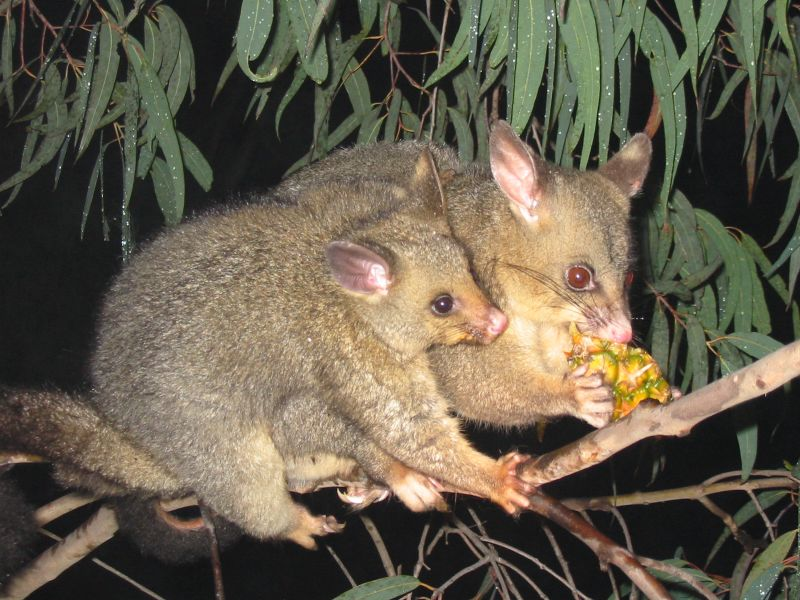
\includegraphics[height=2.8in]{ch1/possumPic/possumPic.jpg} \\
\addvspace{2mm}
\begin{minipage}{\textwidth}
   \caption[possums]{The common brushtail possum of Australia\footnote{Photo by wollombi on Flickr: \texttt{http://flickr.com/photos/wollombi/58499575/}}.}
   \label{possumPic}
\end{minipage}
\end{center}
\end{figure}

\subsection{Variable relationships}
\label{variableRelations}

Many analyses are motivated by a researcher looking for a relationship between two or more variables. A biologist studying possums in the eastern Australia may want to know answers to some of the following questions.
\begin{enumerate}
\item[(1)]\label{questionAboutPossumHeadLengthAndWidth} If a possum has a shorter-than-average head, will its skull width usually be smaller or larger than the average skull width? \label{possumHeadSizeQuestion}
\item[(2)]\label{maleOrFemalePossumsLonger} Will males or females, on average, be longer? \label{possibleCausationQuestionForPossums}
\item[(3)]\label{whichPopulationOfPossumWillBeLargerOnAverage} Which population of possum will be larger on average: Victoria or the other locations they live?
\item[(4)]\label{doesTheProportionOfMalesDifferBasedOnLocation} Does the proportion of males differ based on location, i.e. from Victoria to the other locations?
\end{enumerate}

To answer these questions, data must be collected. Four observations from such a new data set is shown in Table~\ref{possumDF}, and descriptions of each variable are shown in Table~\ref{possumVariables}.
\begin{table}
\begin{center}
\begin{tabular}{ccc ccc cc}
  \hline
& pop & sex & age & headL & skullW & totalL & tailL \\
  \hline
1 & Vic & m & 8 & 94.1 & 60.4 & 89.0 & 36.0 \\
2 & Vic & f & 6 & 92.5 & 57.6 & 91.5 & 36.5 \\
3 & Vic & f & 6 & 94.0 & 60.0 & 95.5 & 39.0 \\
%4 & Vic & f & 2 & 91.5 & 56.3 & 85.5 & 36.0 \\
$\vdots$ & $\vdots$ & $\vdots$ & $\vdots$ & $\vdots$ & $\vdots$ & $\vdots$ & $\vdots$ \\
104 & other & f & 3 & 93.6 & 59.9 & 89.0 & 40.0 \\
   \hline
\end{tabular}
\end{center}
\caption{Four lines from the \data{possum} data set.}
\label{possumDF}
%  xtable(possum[c(1,2,3,104), c(1, 3, 4, 5, 6, 7, 8, 9)], digits=1)
%\end{table}
%\begin{table}
\begin{center}\small
\begin{tabular}{lp{9.5cm}}
\hline
{\bf variable} & {\bf description} \\
\hline
\var{pop} & location where possum was trapped (\resp{Vic} or \resp{other}) \\
\var{sex} & possum's gender (\resp{m} or \resp{f}) \\
\var{age} & age, in years (whole number, data range: \resp{1} to \resp{9}) \\
\var{headL} & head length, in mm (data range: \resp{82.5} to \resp{103.1}) \\
\var{skullW} & skull width, in mm (data range: \resp{50.0} to \resp{68.6}) \\
\var{totalL}  &  total length, in cm (data range: \resp{75.0} to \resp{96.5}) \\
\var{tailL}  &  tail length, in cm (data range: \resp{32.0} to \resp{43.0}) \\
\hline
\end{tabular}
\end{center}
\caption{Variables and their descriptions for the \data{possum} data set.}
\label{possumVariables}
\end{table}

%\begin{exercise} \label{4possumQuestions}
%Guess what the answer might be to each of the four questions above without examining the data.
%\end{exercise}

%\begin{exercise}
%How confident are you about your answers in Exercise~\exer{4possumQuestions}?
%\end{exercise}

Examining summary statistics could provide insights to each of the four questions about possums. Additionally, graphs of the data are useful to answering such questions.
\begin{figure}
   \centering
   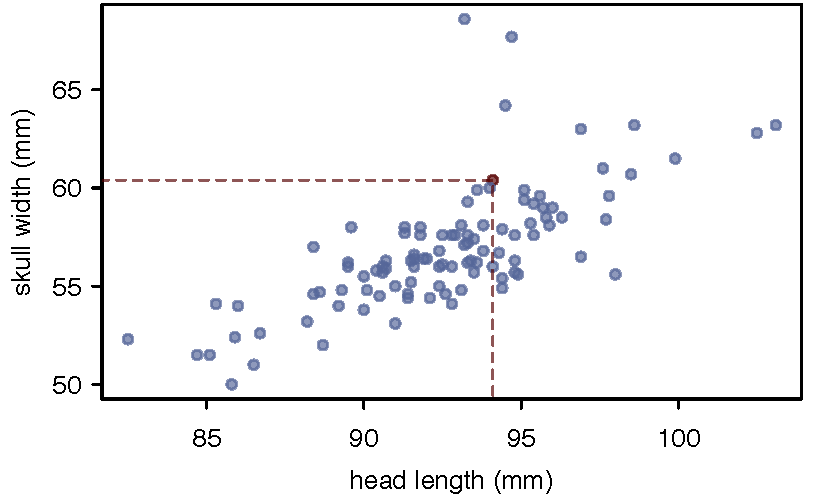
\includegraphics[height=2.5in]{ch1/possumHeadVsSkullW/possumHeadVsSkullW}
   \caption{A scatterplot showing \var{skullW} against \var{headL}. The first possum with a head length of 94.1mm and a skull width of 60.4mm is highlighted.}
   \label{possumHeadVsSkullW}
\end{figure}

Scatterplots are one type of graph used to study the relationship between two variables. Figure~\ref{possumHeadVsSkullW} compares the \var{headL} and \var{skullW} variables. Each point represents a single possum. For instance, the red dot corresponds to Possum~1 from Table~\ref{possumDF}, which has a head length of 94.1mm and a skull width of 60.4mm. The scatterplot suggests that if a possum has a short head, then its skull width also tends to be smaller than the average possum.

\begin{exercise}
Examine the variables in the \data{cars} data set, which are described in Table~\ref{carsVariables} on page~\pageref{carsVariables}. Create two questions about the relationships between these variables that are of interest to you.
%Create two additional questions about the relationships between the variables that are of interest to you.
\end{exercise}

%The first question about \data{possum}, discussed above, is sort of boring. So possums with short heads tend to have slimmer skulls -- that isn't surprising! But some of the other questions might stem from a deeper question.

\subsection{Associated and independent variables}
\label{associatedAndIndependentVariablesSubsection}

The variables \var{headL} and \var{skullW} are said to be \emph{associated} because the plot shows a discernible pattern. When two variables show some connection with one another, they are \term{associated} variables. Associated variables can also be called \term{dependent} variables and vice-versa.

\begin{example}{Examine the scatterplot of \var{weight} and \var{mpgCity} in Figure~\vref{carsMpgCityVsWeight}. Are these variables associated?}
It appears that the heavier a car is, the worse mileage it gets. Since there is some relationship between the variables, they are associated.
\end{example}
\begin{figure}
   \centering
   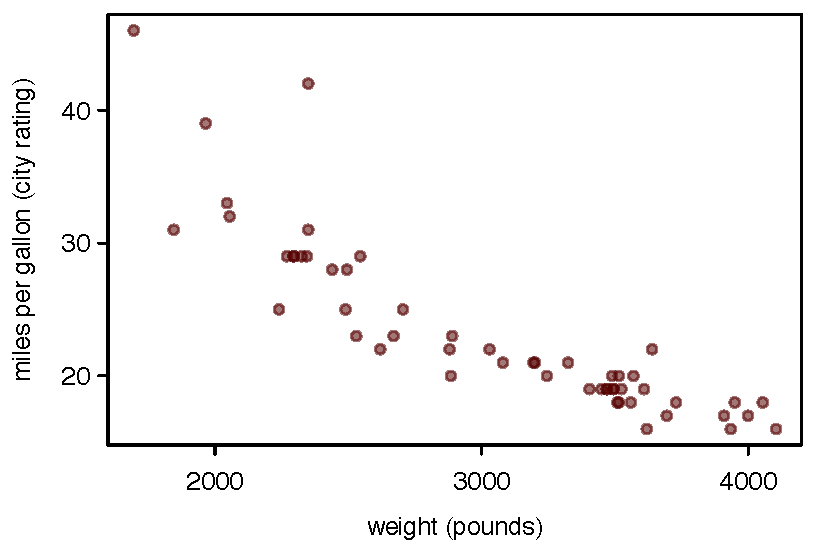
\includegraphics[height=2.6in]{ch1/carsMpgCityVsWeight/carsMpgCityVsWeight}
   \caption{A scatterplot of \var{mpgCity} versus \var{weight} for the \data{cars} data set.}
   \label{carsMpgCityVsWeight}
\end{figure}

Because there is a downward trend in Figure~\ref{carsMpgCityVsWeight} --  larger weights are associated with lower mileage -- these variables are said to be \term{negatively associated}. A \term{positive association} is shown in the possum data represented in Figure~\ref{possumHeadVsSkullW}, where longer heads are associated with wider skulls.

If two variables are not associated, then they are \term{independent}. That is, two variables are independent if there is no evident connection between the two. % In the sulphinpyrazone study, we would like to know if the patients' outcomes are independent of the treatment they received. If they are independent, this would mean the drug does not work. If they are as
It is also possible for cases -- such as a pair of possums or a pair of people -- to be independent. For instance, if possums 1 and 2 do not have any natural connection, such as being siblings or competing for resources in the same territory, then they can be called independent.

% It is also possible for cases or individuals to be independent. For instance, if we randomly pick two possums from Australia,  will not be related 

%\begin{termBox}{\tBoxTitle{Independence}
%Two things are independent of each other if they are not associated (dependent).}
%\end{termBox}

\begin{termBox}{\tBoxTitle{Associated or independent, not both}
A pair of variables are either related in some way (associated) or not (independent). No pair of variables is both associated and independent. These same definitions hold true for a pair of cases as well.}
\end{termBox}

Variables can be associated or independent. Cases can be associated or independent. However, a variable cannot be associated or independent of a case. For example, the \var{headL} variable cannot be independent of possum 1. In statistics, for two things to be independent of each other, they must be comparable. It makes no sense to discuss independence between a variable and a case. 

Association between categorical variables will be discussed in Section~\ref{categoricalData}, and associations between categorical and numerical variables will be discussed specifically in Section~\ref{comparingAcrossGroups}.

%Usually we want our cases to be independent. To this end, we usually take a 

%\begin{example}{A study investigating whether a drug could reduce deaths in heart attack patients was introduced in Section~\ref{}. What we are searching for in the data is whether or not the}


%\subsection{Independence}

%There was no connection between which cars were or were not selected for the \term{cars} data set. They were \term{independently} selected. More formally, these cases are said to be \term{independent} of each other. Independence is a key concept in statistics.

%It is also possible for variables to be independent of one-another. If knowing a car's city mileage provided no information about its price, then \var{mpgCity} and \var{price} are independent variables. \\

%The variables \var{mpgCity} and \var{price} can be independent. Car 35 and car 51 in our sample can be independent. However, the variable \var{price} cannot be independent of car 35. In statistics, for two things to be independent of each other, they must be comparable. It makes no sense to discuss independence between a variable and a case. 

%Even when cases are not explicitly selected at random, such as in the \data{possum} data set, it is common to assume they are independent. Each possum might be equally likely to be caught in the trap, so the trapping itself was used to simulate the random sample. One should always be cautious of these assumptions.

\subsection{Variable types}
\label{variableTypes}

Examine each of the following variables in the \data{cars} data set: \var{type}, \var{price}, \var{driveTrain}, and \var{passengers}. Each of these variables is inherently different from the others yet many of them share certain characteristics.

First consider \var{price}, which is said to be a \term{numerical} variable since the values it takes are numbers and those numbers have a meaningful ordering. That is, all 54 cars could be ordered according to \var{price}, and this ordering would have meaning (e.g. least expensive to most expensive).

The \var{passengers} variable is also numerical, although it seems to be a little different than \var{price}. The variable \var{passengers} can only take whole positive numbers (\resp{1}, \resp{2}, ...) since there isn't a way to have 4.5 passengers. The variable \var{passengers} is said to be \term{discrete} since it only can take numerical values with jumps (e.g. 1, 2, 3, ...). On the other hand, \var{price} is said to be \term{continuous}. % ZZQ: the definition of discrete needs work

The variable \var{driveTrain} can only take a few different values: \resp{front}, \resp{rear}, and \resp{4WD}. Because the responses themselves are categories, \var{driveTrain} is called a \term{categorical} variable\footnote{Sometimes also called a \term{nominal} variable.}. The three possible values (\resp{front}, \resp{rear}, \resp{4WD}) are called the variable's \term{levels}.

Finally, consider the \var{type} variable describing whether a car is \resp{small}, \resp{medium}, or \resp{large}. This variable seems to be a hybrid: it is a categorical variable but the levels have some inherent ordering. A variable with these properties is called an \term{ordinal} variable. To simplify analyses, any ordinal variables in this book will be treated as categorical variables.
\begin{figure}
\centering
\includegraphics[height=1.3in]{ch1/variables/variables}
\caption{Breakdown of variables into their respective types.}
\label{variables}
\end{figure}

\begin{example}{What are the variable types of \var{sex} and \var{headL} in the \data{possum} data set?}
Because the \var{sex} variable takes non-numerical values, it is a categorical variable. Because \var{headL} has numbers as a response and it is meaningful to order these observations by their numbers, it is a numerical variable. More specifically, since \var{headL} can be any length, this variable is a \emph{continuous} numerical variable even though the measured values are all rounded to one decimal.
\end{example}

\begin{exercise}
Identify each of the remaining variables in the \data{possum} data set as either continuous numerical, discrete numerical, or categorical.
\end{exercise}

\begin{exercise}\label{possumSiteExer}
An additional variable was recorded for the \data{possum} data set called \var{site}. Each possum's site is represented a number \resp{1}, \resp{2}, ..., or \resp{7}, however, the ordering of the numbers doesn't actually hold meaning. Is this a numerical or categorical variable? Answer in the footnote\footnote{Because the order of the numbers holds no meaning, this is a categorical variable.}.
\end{exercise}

\section{Examining numerical data}
\label{numericalData}

The \data{cars} data set represents a \emph{sample} from a larger set of cases. This larger set of cases is called the \term{population}. Ideally data would be collected from every case in the population. However, this is rarely possible due to high costs of data collection. As a substitute, statisticians collect subsets of the data called \term{samples} to gain insights into the population. The \data{cars} data set represents a sample of all cars from 1993, and the \data{possum} data set represents a sample from all possums in Australian states of Victoria, New South Wales, and Queensland. In this section we introduce summary statistics and graphics as a first step in analyzing numerical data from a sample to help us understand what is going on in the population as a whole.

\subsection{Scatterplots for paired data}
\label{scatterPlots}

Scatterplots provide an case-by-case view of data for two numerical variables. In Section~\ref{variableRelations}, a scatterplot was informally introduced and used to examine how head length and skull width were related in the \data{possum} data set. Another scatterplot is shown in Figure~\ref{carsPriceVsWeight}, comparing \var{price} and \var{weight} for the \data{cars} data set.
\begin{figure}
   \centering
   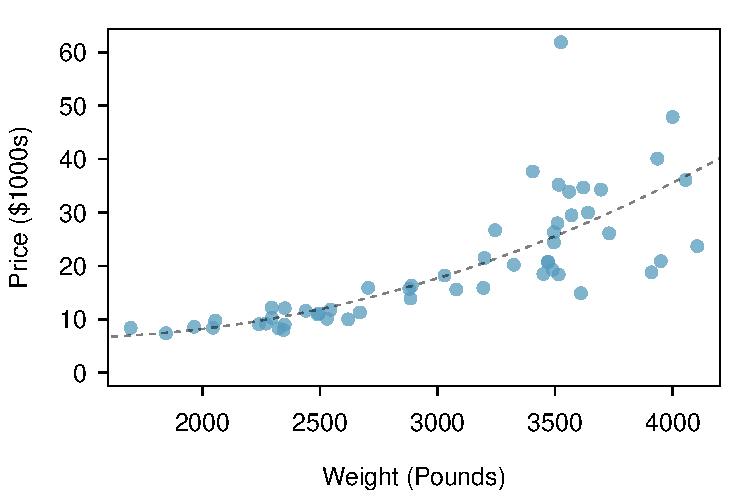
\includegraphics[height=2.6in]{ch1/carsPriceVsWeight/carsPriceVsWeight}
   \caption{A scatterplot of \var{price} versus \var{weight} for the \data{cars} data set.}
   \label{carsPriceVsWeight}
\end{figure}

In any scatterplot, each point represents a single case. Since there are 54 cases in \data{cars}, there are 54 points in Figure~\ref{carsPriceVsWeight}.

\begin{exercise}
What do scatterplots reveal about the data, and how might they be useful?
\end{exercise}

Some associations are more linear, like the relationship between \var{skullW} and \var{headL}, shown in Figure~\ref{possumHeadVsSkullW} on page~\pageref{possumHeadVsSkullW}. Others, like the one seen in Figure~\ref{carsMpgCityVsWeight} on page~\pageref{carsMpgCityVsWeight}, can be curved.

\begin{exercise}
Describe two variables that would have a horseshoe shaped association in a scatterplot. One method to determine such a pair of variables is given in the footnote\footnote{Consider the case where your vertical axis represents something ``good'' and your horizontal axis represents something that is only good in moderation. Health and water consumption fit this description since water becomes toxic when consumed in excessive quantities.}.
\end{exercise}

\subsection{Dot plots and the mean}
\label{dotPlot}

Sometimes two variables is one too many: only one variable may be of interest. In these cases, a dot plot provides the most basic of displays. A dot plot is a one-variable scatterplot, and a sample dot plot is shown in Figure~\ref{carsPriceDotPlot}.
\begin{figure}
   \centering
   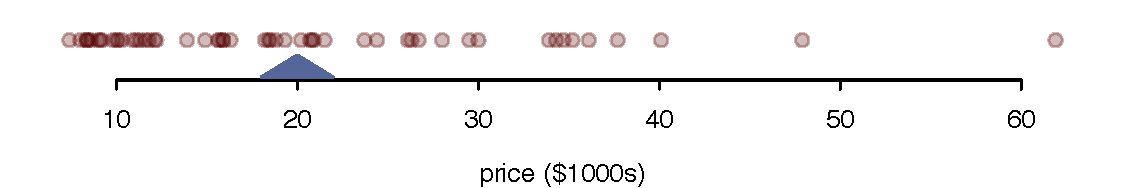
\includegraphics[height=1.3in]{ch1/carsPriceDotPlot/carsPriceDotPlot}
   \caption{A dot plot of \var{price} for the \data{cars} data set. The triangle marks the sample's mean price.}
   \label{carsPriceDotPlot}
\end{figure}

The \term{mean}, sometimes called the average, is a way to measure the center of a \term{distribution} of data. To find the mean price of the cars in the sample, add up all the prices and divide by the number of cases.
\begin{eqnarray}
\bar{x} = \frac{15.9 + 33.9 + \cdots + 26.7}{54} = 19.99259
\label{sampleMeanEquation}
\end{eqnarray}
The sample mean is often labeled $\bar{x}$\marginpar[\hfill $\bar{x}$]{$\bar{x}$}. The letter $x$ is being used as an abbreviation for \var{price}, and the bar says it is the sample average of price. It is useful to think of the mean as the balancing point of the distribution.

\begin{termBox}{\tBoxTitle{Mean}
The sample mean of a numerical variable (continuous or discrete) is computed as the sum of all of the observations divided by the total number of observations:
\begin{eqnarray}
\bar{x} = \frac{x_1+x_2+\cdots+x_n}{n}
\label{meanEquation}
\end{eqnarray}
where $x_1, x_2, \dots, x_n$ represent the $n$ observed values.}
\end{termBox}

\begin{exercise}
Examine equations~(\ref{sampleMeanEquation}) and~(\ref{meanEquation}) above. What does $x_1$ correspond to? And $x_2$? Can you infer a general meaning to what $x_i$ might represent. Answers in the footnote\footnote{$x_1$ corresponds to the price of the first car (15.9), $x_2$ to the price of the second car (33.9), and $x_i$ would correspond to the price of the $i^{th}$ car in the data set.}.
\end{exercise}

\begin{exercise}
What was $n$ in the \data{cars} data set? Answer in the footnote\footnote{The sample size is $n=54$.}.
\end{exercise}

The \emph{population} mean is also computed in the same way, however, it has a special label: $\mu$. The symbol, $\mu$\marginpar[\hfill $\mu$]{$\mu$}, is the Greek letter \emph{mu} and represents the average of all observations in the population. Sometimes a subscript, such as $_x$, is used to represent which variable the population mean refers to, i.e. $\mu_x$.

\begin{example}{The average price of all cars from 1993 can be estimated using the sample data. Based on the \data{cars} sample, what would be a reasonable estimate of $\mu_x$, the mean price of cars from 1993?}
The sample mean may provide a good estimate of $\mu_x$. While this estimate will not be perfect, it provides a \emph{single point estimate} of the population mean.
\end{example}

\subsection{Histograms and shape}
\label{histogramsAndShape}

Dot plots show the exact value for each observation. This is great for small data sets, but can become problematic for larger samples where it is useful to \emph{bin} the data. For example, in the \data{cars} data set, we could create a table of counts for the number of cases with price between \$5,000 and \$10,000, then the number of cases between \$10,000 to \$15,000, and so on. Observations that fall on the boundary of a bin (e.g. \$10,000) are allocated to the lower bin. This tabulation is shown in Table~\ref{binnedCarsPriceTable}. To make the data easier to see visually, these binned counts are plotted as a bar chart in Figure~\ref{carsPriceHist}. When the bins are all of equal width and in consecutive order, the resulting plot is called a \term{histogram}.
\begin{table}[ht]
\begin{center}\small
\begin{tabular}{l ccc ccc ccc}
  \hline
Price & 5-10 & 10-15 & 15-20 & 20-25 & 25-30 & 30-35 & $\cdots$ & 55-60 & 60-65 \\
  \grayline
Count & 11 &  11 &  10 &   7 &   6 &   3 & $\cdots$ & 0 & 1 \\
  \hline
\end{tabular}
\end{center}
\addvspace{-3mm}
\caption{The counts for the binned \var{price} data.}
\label{binnedCarsPriceTable}
\end{table}
\begin{figure}[bth]
   \centering
   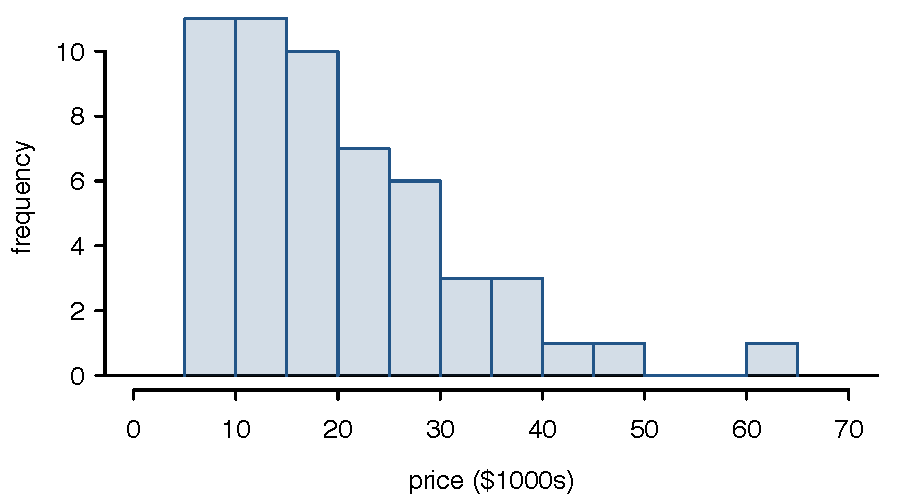
\includegraphics[height=2.3in]{ch1/carsPriceHist/carsPriceHist}
   \caption{Histogram of \var{price}.}
   \label{carsPriceHist}
\end{figure}

Histograms provide a view of the \term{data density}. Higher bars represent where the data is relatively more common. For instance, there are many more cars with a price below \$15,000 than cars that cost at least \$50,000 in the data set. The bars also make it especially easy to see how the data changes from one price to another: in general, the higher the price, the fewer the cars.

Histograms are especially convenient for describing the data's \term{shape}\label{shapeFirstDiscussed}. Figure~\ref{carsPriceHist} shows that most cars have a lower price, while fewer cars have higher prices. When data trails off to the right in this way and has a longer right \hiddenterm{tail}, the shape is said to be \term{skewed to the right}\footnote{Other ways to describe data skewed to the right: \term{right skewed}, \term{skewed to the high end}, or \term{skewed to the positive end}.}.

Data sets with the reverse characteristic -- a long, thin tail to the left -- are said to be \term{left skewed}. It might also be said that such a distribution has a long left tail. Data sets that show roughly equal trailing off in both directions are called \term{symmetric}.

\begin{termBox}{\tBoxTitle{Long tails to identify skew}
When data trails off in one direction, it is called a \term{long tail}. If a distribution has a long left tail, it is left skewed. If a distribution has a long right tail, it is right skewed.}
\end{termBox}

\begin{exercise}
Take a look at Figure~\ref{carsPriceDotPlot} on page~\pageref{carsPriceDotPlot}. Can you see the skew in the data? Is it easier to see the skew in Figure~\ref{carsPriceDotPlot} or Figure~\ref{carsPriceHist}?
\end{exercise}

\begin{exercise}
Besides the mean (since it was labeled), what can you see in Figure~\ref{carsPriceDotPlot} that you cannot see in \ref{carsPriceHist}? Answer in the footnote\footnote{The individual prices.}.
\end{exercise}

In addition to looking at whether a distribution is skewed or symmetric, histograms can be used to identify modes. A \term{mode} is represented by a prominent peak in the distribution\footnote{Another definition of mode, which is not typically used in statistics, is the value with the most occurrences. It is common to have \emph{no} observations with the same values in a data set, which makes this other definition useless for many real data sets.}. There is only one prominent peak in the histogram of \var{price}. % students could learn about bin size selection here. however, maybe we want to postpone this idea until we incorporate kernel smoothing and have a bias-variance discussion.

Figure~\ref{singleBiMultiModalPlots} shows histograms that have one, two, and three prominent peaks. Such distributions are called \term{unimodal}, \term{bimodal}, and \term{multimodal}, respectively. Any distribution with more than 2 prominent peaks is called multimodal. Notice that there was one prominent peak in the unimodal distribution with a second less prominent peak that was not counted since it only differs from its neighboring bins by a few observations.
\begin{figure}
   \centering
   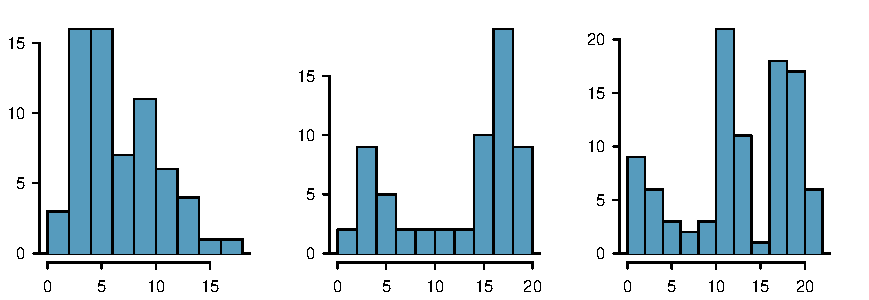
\includegraphics[height=1.8in]{ch1/singleBiMultiModalPlots/singleBiMultiModalPlots}
   \caption{Counting only prominent peaks, the distributions are (left to right) unimodal, bimodal, and multimodal.}
   \label{singleBiMultiModalPlots}
\end{figure}

\begin{exercise}
Figure~\ref{carsPriceHist} reveals only one prominent mode in \var{price}. Is the distribution unimodal, bimodal, or multimodal?
\end{exercise}

\begin{exercise}
Height measurements of everyone at a K-2 elementary school were taken, which includes only young students and adult teachers. How many modes would you anticipate in this height data set? Answer in the footnote\footnote{There might be two height groups visible in the data set: one of the students and one of the adults. That is, the data might be bimodal.}.
\end{exercise}

\begin{tipBox}{\tipBoxTitle{Looking for modes}
Looking for modes isn't about a clear and correct answer about the number of modes in a distribution, which is why \emph{prominent} is not defined mathematically here. The importance of this examination is to better understand your data and how it might be structured.}
\end{tipBox}

If you find two or more prominent peaks, the data may arise from two or more subpopulations. Even if the distribution is not bimodal or multimodal, it is certainly not uncommon to reap benefits from grouping data by other variables, which will be discussed casually in Section~\ref{comparingAcrossGroups}.

\subsection{Variance and standard deviation}
\label{variability}

The mean was introduced as a method to describe the center of a data set but the data's variability is also important. Here two measures of variability are introduced: the variance and the standard deviation. Both of these are very useful in data analysis, even though their formulas are a bit tedious to compute by hand.

We call the distance of an observation from its mean its \term{deviation}. Below are the $1^{st}_{}$, $2^{nd}_{}$, and $54^{th}_{}$ deviations for the \var{price} variable:
\begin{eqnarray*}
&& x_1^{}-\bar{x} = 15.9-20 = -4.1 \hspace{5mm}\text{ } \\
&& x_2^{}-\bar{x} = 33.9-20 = 13.9 \\
&& \vdots \\
&& x_n^{}-\bar{x} = 26.7-20 = 6.7
\end{eqnarray*}
If we square these deviations and then take an average, the result is about equal to the sample \term{variance}\label{varianceIsDefined}, denoted by $s_{}^2$\marginpar[\hfill $s_{}^2$]{$s^2_{}$}:
\begin{eqnarray*}
s_{}^2 = \frac{(-4.1)_{}^2 + (13.9)_{}^2 + (6.7)_{}^2}{54-1} = \frac{16.8 + 193.2 + 44.9}{53} = 132.4
\end{eqnarray*}
We divide by $n-1$ instead of $n$ for reasons described in the footnote\footnote{The population of all cars from 1993 has some precise variance in \var{price}. Our estimate of this variance tends to be slightly better if we divide by $n-1$ instead of $n$.}. Notice that squaring the deviations does two things: (i) it makes large values much larger, seen by comparing $(-4.1)^2$, $13.9^2$, and $6.7^2$, and (ii) it gets rid of any negative signs.

The \term{standard deviation} is defined as the square root of the variance: $s=\sqrt{132.4} = 11.5$\marginpar[\hfill $s_{}^{}$]{$s_{}^{}$}. If we like, a subscript of $_x$ may be added to the the variance and standard deviation -- that is, $s_x^2$ and $s_x^{}$ -- as a reminder that these are the variance and standard deviation of the observations represented by $x_1^{}$, $x_2^{}$, ..., $x_n^{}$. These may be omitted when it is clear what the standard deviation is referencing.

\begin{termBox}{\tBoxTitle{Variance and standard deviation}
The variance is roughly the average squared distance from the mean. The standard deviation is the square root of the variance.}
\end{termBox}

Computing the variance and standard deviation for a population uses the same formulas and methods as for a sample. However, like the mean, the population values have special symbols: $\sigma_{}^2$\marginpar[\hfill $\sigma^2_{}$]{$\sigma^2_{}$} for the variance and $\sigma$\marginpar[\hfill $\sigma$]{$\sigma$} for the standard deviation. The symbol $\sigma$ is the Greek letter \emph{sigma}. As with the sample variance and standard deviation, subscripts such as $_{x}^{}$ can be added to specify what the population variance and standard deviation represent.
\begin{figure}
\centering
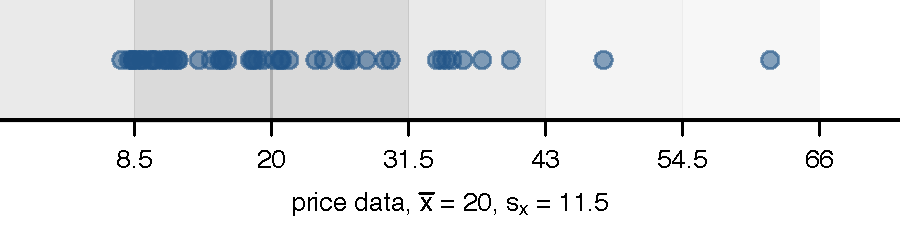
\includegraphics[height=3cm]{ch1/sdAsRuleForCarsPrice/sdAsRuleForCarsPrice}
\caption{In the \var{price} data, 40 of 54 cars (74\%) are within 1 standard deviation of the mean, \$20,000. Additionally, 52 of the 54 cars (96\%) and 53 of the 54 prices (98\%) are within 2 and 3 standard deviations, respectively.}
\label{sdAsRuleForCarsPrice}
\end{figure}

The standard deviation is useful in considering how close the data is to the mean. Usually about 70\% of the data is within one standard deviation of the mean and 95\% within two standard deviations. However, these percentages can and do vary from one distribution to another. Figure~\ref{severalDiffDistWithSdOf1} shows several different distributions that have the same center and variability but very different shapes.
\begin{figure}
\centering
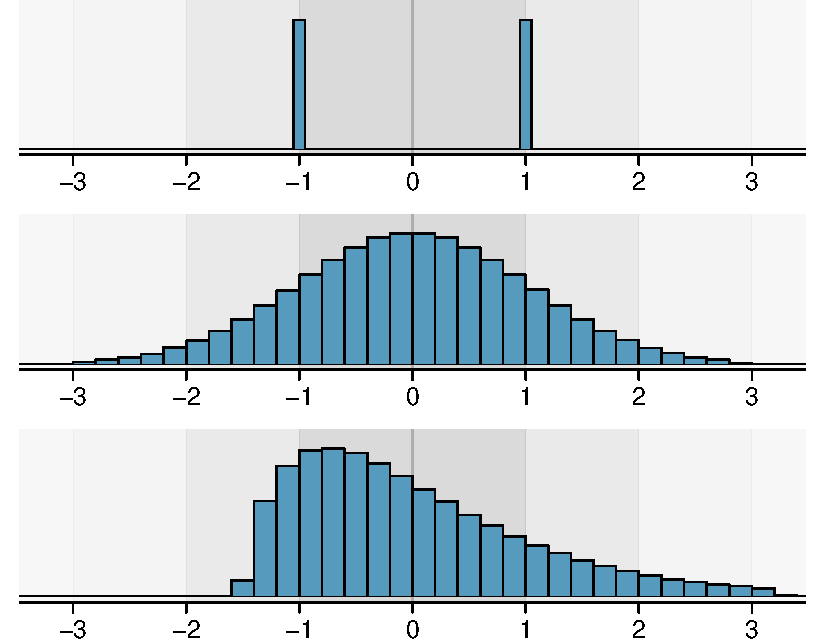
\includegraphics[width=105mm]{ch1/severalDiffDistWithSdOf1/severalDiffDistWithSdOf1}
\caption{Three very different population distributions with the same mean $\mu=0$ and standard deviation $\sigma=1$.}
\label{severalDiffDistWithSdOf1}
\end{figure}

\begin{exercise}
On page~\pageref{shapeFirstDiscussed}, the concept of distribution shape was introduced. A description of the shape of a distribution should include modality and whether the distribution is symmetric or skewed to one side. Using Figure~\ref{severalDiffDistWithSdOf1} as an example, explain why such a description is important.
\end{exercise}

\begin{example}{Describe the distribution of the \var{price} variable, shown in a histogram on page~\pageref{carsPriceHist}. The description should incorporate the center, variability, and shape of the distribution, and it should also be placed in context of the problem: the price of cars. Also note any especially interesting cases.}
The distribution of car prices is unimodal and skewed to the high end. Many of the prices fall near the mean at \$20,000, and most fall within one standard deviation (\$11,500) of the mean. There is one very expensive car that costs more than \$60,000.
\end{example}

%; a very peculiar distribution might have no data within one standard deviation or only 75\% of the data within two standard deviations. %, For instance, it is guaranteed that no more than $\frac{1}{2^2}=1/4^{th}$ of the data will be further than 2 standard deviations from the mean. Likewise, at most $\frac{1}{3^2}=1/9^{th}$ of the data can be further than 3 standard deviations. The Theorem in the footnote provides the general rule\footnote{Chebyshev's Theorem: No more than a fraction $1/k^2$ of the data can be further than $k$ standard deviations from the mean. This rule is conservative for many data sets.}.

%These approximate guidelines do not give the only use of the standard deviation (and variance), however, the other applications are too obscure to go into detail here. 
In practice, the variance and standard deviation are sometimes used as a means to an end, where the ``end'' is being able to accurately estimate the uncertainty associated with a sample's estimate. For example, in Chapter~4 %ZZQ \ref{foundationsForInference}
we use the variance and standard deviation to assess how close the sample mean is to the population mean.

\begin{tipBox}{\tipBoxTitle{standard deviation describes variability}
Standard deviation is complex mathematically. However, it is not conceptually difficult. %: it provides a useful measure of the variability in a data set.
It is useful to remember that usually about 70\% of the data is within one standard deviation of the mean and about 95\% is within two standard deviations.}
\end{tipBox}


%This rule does not provide the only use of the standard deviation, which provides a solid foundation for understanding variability in the data. In practice, the variance and standard deviation are many times a means to an end, and the ``end'' is being able to accurately estimate the uncertainty associated with an estimate. For example, the variance and standard deviation are useful in determining how close one should anticipate the sample mean is to the population mean. We will continue to be discuss variance and standard deviation over the next few chapters while the details of its common use will be introduced in Chapter~\ref{foundationsForInference} and beyond.

\subsection{Box plots, quartiles, and the median}

A box plot summarizes a data set using five statistics while also plotting unusual observations. Figure~\ref{boxPlotLayout} provides a vertical dot plot alongside a box plot of the \var{price} variable from \data{cars}.
\begin{figure}[bth]
   \centering
   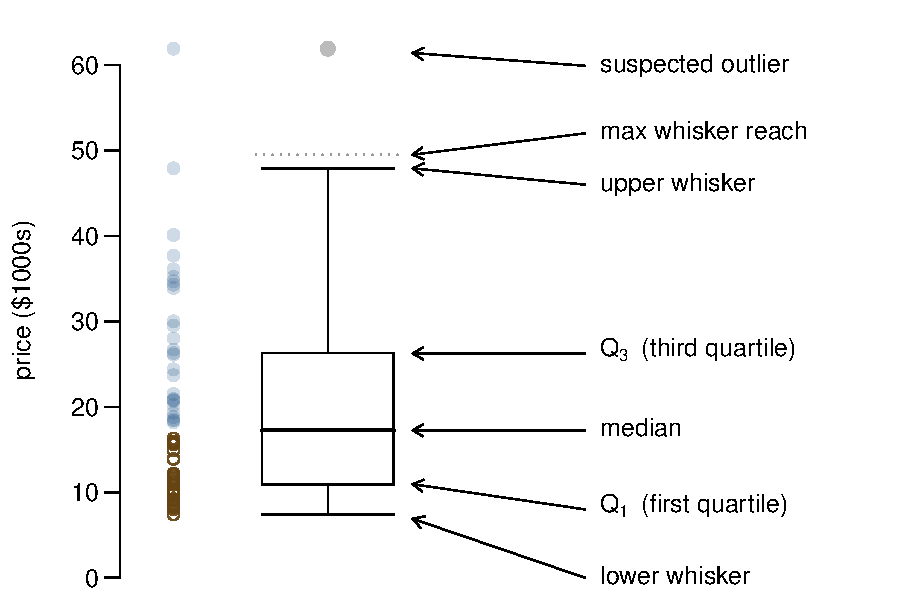
\includegraphics[height=2.8in]{ch1/boxPlotLayout/boxPlotLayout}
   \caption{A vertical dot plot next to a labeled box plot of the \var{price} data. The median (\$17,250), splits the data into the bottom 50\% and the top 50\%, marked in the dot plot by dark-colored hollow circles and light filled circles, respectively.}
   \label{boxPlotLayout}
\end{figure}

The first step in building a box plot is drawing a rectangle to represent the middle 50\% of the data. The total length of the box, which is the vertical distance in Figure~\ref{boxPlotLayout}, is called the \term{interquartile range} (IQR, for short). It, like the standard deviation, is a measure of variability in data. The more variable the data, the larger the standard deviation and IQR. The two boundaries of the box are called the \term{first quartile} (the $25^{th}$ \hiddenterm{percentile}, i.e. 25\% of the data falls below this value) and the \term{third quartile} (the $75^{th}$ percentile), and these are often labeled $Q_1$ and $Q_3$, respectively.

\begin{termBox}{\tBoxTitle{Interquartile range (IQR)}
The \term{interquartile range (IQR)} is the length of the box in box plot. It is computed as
\begin{eqnarray*}
IQR = Q_3 - Q_1
\end{eqnarray*}
where $Q_1$ and $Q_3$ are the $25^{th}$ and $75^{th}$ percentiles.}
\end{termBox}

%\begin{exercise}
%The first quartile is also the $25^{th}$ \term{percentile} and the third quartile is the $75^{th}$ percentile. What does \term{percentile} mean? How many of the observations would fall below the $50^{th}$ percentile? Answers in the footnote\footnote{The  For example, the $25^{th}$ percentile is the value where 25\% of the data is below and 75\% above. The $50^{th}$ percentile is the value where half of the data is below and half above.}.
%\end{exercise}

The line splitting the box marks the \term{median}, or the value that splits the data in half. Figure~\ref{boxPlotLayout} shows 50\% of the data falling below the median (dark hollow circles) and other 50\% falling above the median (light-colored filled circles). There are 54 car prices in the data set so the data is perfectly split into two groups. We take the median in this case to be the average of the two observations closest to the $50^{th}$ percentile: $\frac{\$16,300 + \$18,200}{2} = \$17,250$. When there are an odd number of observations, there will be exactly one observation that splits the data into two halves, and in this case that observation is the median (no average needed).

%The line splitting the box marks the \term{median}, or the ``middle'' observation in the data. Half of the observations fall below the median and half are above. In the \data{cars} data set, there are 54 car prices, in which case  in the data set and the $27^{th}$ and $28^{th}$ largest observations (the middle observations) are \$16,300 and \$18,200. Because this represents a tie for the middle number, the median is taken as the average of the two: \$17,250. \\


\begin{termBox}{\tBoxTitle{Median: the number in the middle}
If the data was ordered from smallest to largest, the \term{median} would be the observation right in the middle. If there are an even number of observations, there will be two values in the middle, and the median is taken as their average.}
\end{termBox}

\begin{exercise}
How much of the data falls between $Q_1$ and the median? How between the median and $Q_3$? Answers in the footnote\footnote{Since $Q_1$ and $Q_3$ capture the middle 50\% of the data and the median splits the middle of the data, 25\% of the data falls between $Q_1$ and the median, and another 25\% falls between the median and $Q_3$.}.
\end{exercise}

Extending out from the box, the \term{whiskers} attempt to capture the data outside of the box, however, their maximum reach is only $1.5*IQR$.\footnote{While the choice of exactly 1.5 is arbitrary, it is the most commonly used value for box plots.} They grab everything within this reach. In Figure~\ref{boxPlotLayout}, the upper whisker cannot extend to the last point, which is beyond $Q_3 + 1.5*IQR$, and so extends only to the last point below this limit. The lower whisker stops at the lowest price, \$7,400, since there is no additional data to reach. In a sense, the box is like the body of the box plot and the whiskers are like its arms trying to reach the rest of the data.

Any observation that lies beyond the whiskers is labeled with a dot. The purpose of labeling these points -- instead of just extending the whiskers to the minimum and maximum observed values -- is to help identify any observations that appear to be unusually distant from the rest of the data. Unusually distant observations are called \term{outliers}. In the case of the \var{price} variable, the car with price \$61,900 is a potential outlier.

\begin{termBox}{\tBoxTitle{Outliers are extreme}
An \term{outlier} is an observation that appears extreme relative to the rest of the data.}
\end{termBox}

Examination of data for possible outliers serves many useful purposes, including
\begin{enumerate}
\item identifying extreme skew in the distribution.
\item finding evidence that extreme cases are common for the variable being examined.
\item identifying data collection or entry errors. If there was car price listed as \$140,000, it is worth reviewing the observation to see whether it was really \$14,000.
\item providing insights into interesting phenomena with the data.
\end{enumerate}

\begin{tipBox}{\tipBoxTitle{Why it is important to look for outliers}
The identification of outliers is not actually what is important, which is why no rigid definition for outlier is provided. What is important is to examine and take special note of \emph{suspected} outliers and why they are extreme from the rest of the data.}
\end{tipBox}

\begin{exercise}
The observation \$61,900, a suspected outlier, was found to be an accurate observation. What would such an observation suggest about the nature of vehicle prices?
\end{exercise}

\begin{exercise}
Using Figure~\vref{boxPlotLayout}, estimate the following values for \var{price} in the \data{cars} data set: (a) $Q_1$, (b) $Q_3$, (c) IQR, and (d) the maximum length of the upper whisker. How are (c) and (d) related?
\end{exercise}

\subsection{Robust statistics}

How would sample statistics be affected if \$200,000 was observed instead of \$61,900 for the most expensive car? Or what if \$200,000 had been in the sample instead of the cheapest car at \$7,400? These two case are plotted alongside the original data in Figure~\ref{carsPriceDotPlotRobustEx}, and sample statistics are computed under each of these scenarios in Table~\ref{robustOrNotTable}.
\begin{figure}
\begin{center}
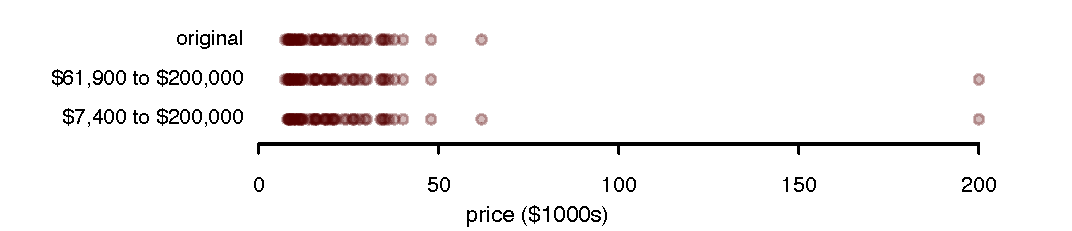
\includegraphics[width=6in]{ch1/carsPriceDotPlotRobustEx/carsPriceDotPlotRobustEx}
\caption{Dot plots of the original price data and two modified price data sets.}
\label{carsPriceDotPlotRobustEx}
\end{center}
\end{figure}
\begin{table}
\begin{center}
\begin{tabular}{l c cc c cc}
  \hline
& \hspace{0mm} & \multicolumn{2}{c}{\bf robust} & \hspace{2mm} & \multicolumn{2}{c}{\bf not robust} \\
scenario && median & IQR && $\bar{x}$ & $s$ \\ 
  \hline
original \var{price} data && 17.25 & 15.30 && 19.99 & 11.51 \\ 
move \$61,900 to \$200,000 && 17.25 & 15.30 && 22.55 & 26.53 \\ 
move \$7,400 to \$200,000 && 18.30 & 15.45 && 26.12 & 35.79 \\ 
   \hline
\end{tabular}
\end{center}
\caption{A comparison of how the median, IQR, mean ($\bar{x}$), and standard deviation ($s$) change when extreme observations are in play.}
\label{robustOrNotTable}
\end{table}

\begin{exercise}
(a) Which is more affected by extreme observations, the mean or median? Table~\ref{robustOrNotTable} may be helpful. (b) Is the standard deviation or IQR more affected by extreme observations?.
\end{exercise}

The median and IQR are called \term{robust estimates} because extreme observations have little effect on their values. The mean and standard deviation are much more affected by changes in extreme observations.

\begin{exercise}
Why doesn't the median or IQR change from the original \var{price} data to the second scenario of Table~\ref{robustOrNotTable}?
\end{exercise}

%\begin{exercise}
%Are the extreme changes in the mean and standard deviation a fluke? Look back to how the mean and standard deviation are actually computed on pages~\pageref{meanEquation} and~\pageref{varianceIsDefined}. Why is it that these two variables are affected by (suspected) outliers, i.e. observations that are far from the rest of the data? Compare this with how the median and IQR are computed.
%\end{exercise}

\begin{exercise}
Why are robust statistics useful? If you were searching for a new car and cared about price, would you be more interested in the mean vehicle price or the median vehicle price when deciding what price you should pay for a regular car?
\end{exercise}

\section{Considering categorical data}
\label{categoricalData}

\subsection{Contingency tables}

Table~\ref{typeDriveTrainTableTotals} summarizes the variables \var{type} and \var{driveTrain} in a single table called a contingency table. \term{Contingency tables} are used to organize two categorical variables, where the counts in the table represent the number of times each combination was observed. For example, there were 19 cars classified as \var{type} = \resp{small} and \var{driveTrain} = \resp{front} of the 54 cars. Row and column totals are also included. The \term{row totals} equal the total counts across each row (e.g. $19+0+2=21$), and \term{column totals} are total counts down each column.
\begin{table}[ht]
\begin{center}
\begin{tabular}{l | ccc | r}
  \hline
 & front & rear & 4WD & total \\ 
  \hline
small &  19 &   0 & 2 & 21 \\ 
midsize &  17 &  5 & 0 & 22 \\ 
large &   7 &   4 & 0 & 11 \\ 
   \hline
total & 43 & 9 & 2 & 54 \\
   \hline
\end{tabular}
\end{center}
\caption{A contingency table for \var{type} and \var{driveTrain}.}
\label{typeDriveTrainTableTotals}
\end{table}

A table for a single variable is called a \term{frequency tables}. A frequency table for \var{type} is shown in Table~\ref{typeContTable}. If we replaced the counts with percentages or proportions, the table would be called a \term{relative frequency table}. \\
\begin{table}[htb]
\begin{center}
\begin{tabular}{ccc}
  \hline
small & midsize & large \\ 
  \hline
21 &  22 &  11 \\ 
   \hline
\end{tabular}
\end{center}
\caption{A frequency table for the \var{type} variable.}
\label{typeContTable}
\end{table} % xtable(matrix(table(cars[,c('type')])[c(4,3,2)], nrow=1))

\begin{exercise}
Examine Tables~\ref{typeContTable} and~\ref{typeDriveTrainTableTotals}. Why is Table~\ref{typeContTable} redundant if Table~\ref{typeDriveTrainTableTotals} is provided?
\end{exercise}

\subsection{Bar charts and proportions}

A bar chart is a common way to display a single categorical variable. The left panel of Figure~\ref{typeBarPlot} shows a \term{bar plot} of \var{type}. In the right panel, the counts were converted into proportions (e.g. $21/54=0.389$ for \var{small}), making it easy to compare how often different outcomes occur irrespective of sample size.
\begin{figure}[bht]
   \centering
   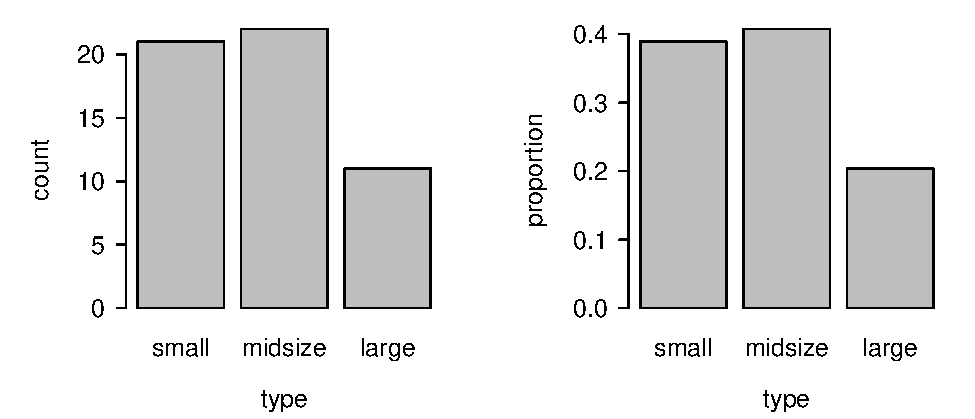
\includegraphics[height=2.3in]{ch1/typeBarPlot/typeBarPlot}
   \caption{Two bar plots of \var{type}. The left panel shows the counts and the right panel the proportions in each group.}
   \label{typeBarPlot}
\end{figure}

\begin{exercise}
Which of the following statements would be more useful to an auto executive? (1) 21 cars in our sample were \resp{small} vehicles. (2) 38.9\% of the cars in our sample were \resp{small} vehicles. Comment in the footnote\footnote{Even if the sample size (54) was provided in the first statement, the auto exec would probably just be trying to figure out the proportion in her head.}.
\end{exercise}

\begin{tipBox}{\tipBoxTitle{data set notation}
Sometimes the values \resp{1} and \resp{0} are used as the outcomes for a categorical variable if it only has two levels. For instance, if there were only \resp{small} and \resp{large} cars, we could have used \resp{1} to represent \resp{small} and \resp{0} to represent \resp{large} in the \var{type} variable.}
\end{tipBox}

If proportions are so great, why not just change Table~\ref{typeDriveTrainTableTotals} into a table of proportions? Because there is a better way. %If there is a two variable contingency table, the relationship between the variables can be examined.

Table~\ref{rowPropTypeDriveTrain} shows the row proportions for Table~\ref{typeDriveTrainTableTotals}. The \term{row proportions} are computed as the counts divided by their row totals. The count 17 at the intersection of \resp{midsize} and \resp{front} is replaced by $17/22=0.773$, i.e. 17 divided by its row total, 22. So what does 0.773 represent? It corresponds to the proportion of \resp{midsize} vehicles in the sample that have front wheel drive.
\begin{table}[ht]
\begin{center}
\begin{tabular}{l | rrr | r}
  \hline
 & front & rear & 4WD & total \\ 
  \hline
small &  $19/21=0.905$ &  $0/21 = 0.000$ & $2/21 = 0.095$   & 1.000 \\ 
midsize &  $17/22 = 0.773$ &  $5/22 = 0.227$ & $0/22=0.000$ & 1.000 \\ 
large &  $7/11 = 0.636$  &   $4/11 = 0.364$  & $0/11=0.000$ & 1.000 \\ 
   \hline
total & $43/54=0.796$ & $9/54=0.167$ & $2/54 = 0.037$ &  1.000 \\
   \hline
\end{tabular}
\end{center}
\caption{Row standardized contingency table for \var{type} and \var{driveTrain}. The proportions are computed as the original counts divided by the row totals.}
\label{rowPropTypeDriveTrain}
\end{table}

A contingency table of the column proportions is computed in a similar way, where each \term{column proportion} is computed as the count divided by the corresponding column total. Table~\ref{colPropTypeDriveTrain} shows such a table. Now the proportions have a different meaning. For example, 0.442 represents the proportion of front wheel drive cars in the sample that that are small cars.
\begin{table}[ht]
\begin{center}
\begin{tabular}{l | rrr | r}
  \hline
 & front & rear & 4WD & total \\ 
  \hline
small &  $19/43=0.442$ &  $0/9 = 0.000$  & $2/2=1.000$ & $21/54=0.389$ \\ 
midsize &  $17/43 = 0.395$ &  $5/9 = 0.556$ & $0/2 = 0.000$ & $22/54=0.407$ \\ 
large &  $7/43 = 0.163$  &   $4/9 = 0.444$  & $0/2 = 0.000$ & $11/54=0.204$ \\ 
   \hline
total & 1.000 & 1.000 & 1.000 & 1.000 \\
   \hline
\end{tabular}
\end{center}
\caption{Column standardized contingency table for \var{type} and \var{driveTrain}. The proportions are computed as the original counts divided by the column totals.}
\label{colPropTypeDriveTrain}
\end{table}

\begin{exercise}
What does 0.364 represent in Table~\ref{rowPropTypeDriveTrain}? Answer in the footnote\footnote{0.364 represents the proportion of large cars in the sample that are rear wheel drive.}. What does 0.444 represent in Table~\ref{colPropTypeDriveTrain}?
\end{exercise}

\begin{exercise}
What does 0.796 represent in Table~\ref{rowPropTypeDriveTrain}? Answer in the footnote\footnote{0.827 represents the proportion of cars in the sample that are front wheel drive vehicles.}. What does 0.407 represent in the Table~\ref{colPropTypeDriveTrain}?
\end{exercise}

\begin{exercise} \label{weighingRowColumnProportions}
Researchers suspect \var{pop} (living location) might be associated with \var{sex} in the \data{possum} data set, and Table~\ref{possumPopSexContTable} is a contingency table for this data. Based on these researchers' interests, which do you think would be more interesting: row or column proportions? Answer in the footnote\footnote{The interest lies in how the \var{sex} changes based on \var{pop}. This corresponds to the row proportions here: the proportion of males/females in each location.}.
\end{exercise}

%\begin{exercise}
%Table~\ref{possumPopSexContTable} is a contingency table for the \data{possum} data set for the \var{pop} (living location) and \var{sex} variables. Which variable makes more sense as an explanatory variable? Answer in the footnote\footnote{It makes more sense for living location to affect the proportion of males to females in the population. The reverse cannot be entirely ruled out: it might be that possums migrate based on gender, although this seems less likely.}.
%\end{exercise}

%\begin{exercise} \label{weighingRowColumnProportions}
%If \var{pop} (living location) is the explanatory variable and \var{sex} the response, which do you think would be more interesting: row or column proportions? Answer in the footnote\footnote{The interest lies in how the response changes based on the explanatory variable. This corresponds to the row proportions here: the proportion of males/females in each location.% The column proportions correspond to what proportion of the sampled females and males are in each region. (If you need convincing that these are the actual meanings of the row and column proportions in these cases, construct each row and column proportion table.% You can do so in R by using the commands \rcom{prop.table(table(possum[,c('pop', 'sex')]), 1)} and \rcom{prop.table(table(possum[,c('pop', 'sex')]), 2)} after loading the data in R -- see Section~\ref{introductoryMethodsInR}.
%)}.
%\end{exercise}
\begin{table}[ht]
\begin{center}
\begin{tabular}{l cc r}
  \hline
 & f & m & total \\ 
  \hline
Vic &  24 &  22 & 46 \\ 
  other &  19 &  39 & 58 \\ 
   \hline
total & 43 & 61 & 104 \\
   \hline
\end{tabular}
\end{center}
\caption{A contingency table for \var{pop} and \var{sex} from the \data{possum} data set.}
\label{possumPopSexContTable}
\end{table}

Exercise~\exer{weighingRowColumnProportions} points out that row and column proportions are not created equal. It is important to consider each before settling on one to ensure that the most useful table is constructed.

\subsection{Mosaic plots and independence}
\label{mosaicPlotsAndIndependence}

Contingency tables using row or column proportions are especially useful for examining how two categorical variables are related. Mosaic plots provide a way to put these tables in a graphical form. To reduce complexity, this section we will only consider vehicles with front and rear wheel drive, as shown in Tables~\ref{typeDriveTrainTableTotalsMinus4wd}(a).
\begin{table}
\begin{center}
\begin{tabular}{l cc r  c l cc}
   \cline{1-4}\cline{6-8}
 & front & rear & total & \hspace{1cm} & & front & rear \\ 
   \cline{1-4}\cline{6-8}
small &  19 &   0 & 19  & & small &  1.00 &   0.00\\ 
midsize &  17 &  5 & 22 & & midsize &  0.77 & 0.23 \\ 
large &   7 &   4 & 11  & & large &   0.64 &  0.36\\ 
   \cline{1-4} \cline{6-8}
total & 43 & 9 & 52  & & total & 0.83 & 0.17\\
   \cline{1-4} \cline{6-8}
 &&&&&&&  \\
   \multicolumn{4}{c}{(a)} && \multicolumn{3}{c}{(b)}
\end{tabular}
\end{center}
\vspace{-6.5mm}
\caption{(a) Contingency table for \var{type} and \var{driveTrain} with the two vehicles with \var{driveTrain} = \resp{4WD} removed. (b) Row proportions for this table.}
\label{typeDriveTrainTableTotalsMinus4wd}
\end{table}

%\begin{table}[ht]
%\begin{center}
%\begin{tabular}{l cc r}
%  \hline
% & front & rear & total \\ 
%  \hline
%small &  19 &   0 & 19 \\ 
%midsize &  17 &  5 & 22 \\ 
%large &   7 &   4 & 11 \\ 
%   \hline
%total & 43 & 9 & 52 \\
%   \hline
%\end{tabular}
%\end{center}
%\caption{A contingency table for \var{type} and \var{driveTrain} with the two vehicles with \var{driveTrain} = \resp{4WD} removed.}
%\label{typeDriveTrainTableTotalsMinus4wd}
%\end{table}

%\begin{exercise} \label{rowPropExerOfTypeDT}
%Create the contingency table of Table~\ref{typeDriveTrainTableTotalsMinus4wd} showing the row proportions. Answer in the footnote\footnote{The last column has been omitted since all values are 1.00.
%\begin{center}
%\begin{tabular}{l cc}
%  \hline
% & front & rear \\ 
%  \hline
%small &  1.00 &   0.00 \\ 
%midsize &  0.77 & 0.23 \\ 
%large &   0.64 &  0.36 \\ 
%   \hline
%total & 0.83 & 0.17 \\
%   \hline
%\end{tabular}
%\end{center}}.
%\end{exercise}

A \term{mosaic plot} is a graphically display of contingency table information. Here we construct the mosaic plot representing the row proportions of \var{type} and \var{driveTrain} in Table~\ref{typeDriveTrainTableTotalsMinus4wd}(b).
\begin{figure}
   \centering
   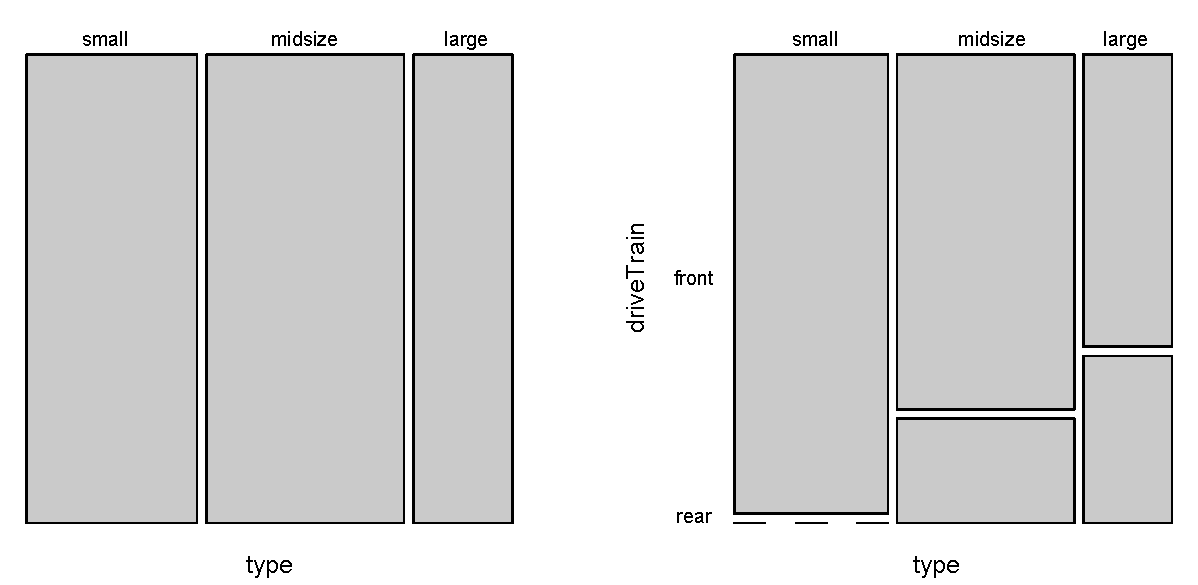
\includegraphics[height=2.2in]{ch1/typeDriveTrainMosaicPlot/typeDriveTrainMosaicPlot}
   \caption{The one-variable mosaic plot for \var{type} and the two-variable mosaic plot for both \var{type} and \var{driveTrain}.}
   \label{typeDriveTrainMosaicPlot}
\end{figure}

The left panel of Figure~\ref{typeDriveTrainMosaicPlot} shows a mosaic plot of \var{type} constructed by vehicle type. Each column represents a level of \var{type}, and the column width corresponds to the proportion of cars of each type. For instance, there were fewer small cars than midsize cars, so the small car column is slimmer.

This plot is further broken into pieces in the right panel using the \var{driveTrain} variable. Each column is split proportionally according to the drivetrain of the vehicles of that particular type. For example, the first column representing only small cars was broken into small cars with front and rear drivetrains. %In the right of Table~\ref{typeDriveTrainTableTotalsMinus4wd}, the proportion of each \var{driveTrain} level was computed within \resp{small}, \resp{midsize}, and \resp{large} cars separately. Similarly, we break apart each of the columns in the left panel of Figure~\ref{typeDriveTrainMosaicPlot} into cars with \resp{front} and \resp{rear} drive trains, which results in the right panel.
As another example, the top of the middle column represents {midsize} cars with front wheel drive, and the lower part of the middle column represents {midsize} cars with rear wheel drive. Because each column is broken apart in very different places, this suggests the proportion of vehicles with front wheel drive differs with vehicle \var{type}. That is, \var{driveTrain} and \var{type} are associated.

In a similar way, a mosaic plot representing column proportions of Table~\ref{typeDriveTrainTableTotals} can be constructed, which is shown in Figure~\ref{driveTrainTypeMosaicPlot}.

%\begin{exercise}
%What does the mosaic plot on the right of Figure~\ref{typeDriveTrainMosaicPlot} suggest about how a vehicle's \var{type} and \var{driveTrain} are related? Answer in the footnote\footnote{It appears that the larger the vehicle, the more likely it is to have a rear drive train. Do you think this result (that larger vehicles are more likely to have rear drive trains) means a vehicle being larger \emph{causes} the vehicle to have rear wheel drive? This question will be answered in Section~\ref{experiments}.}.
%\end{exercise}

\begin{figure}[hht]
   \centering
   \includegraphics[height=2.2in]{ch1/driveTrainTypeMosaicPlot/driveTrainTypeMosaicPlot}
   \caption{Mosaic plot where type is broken up within the drivetrain.}
   \label{driveTrainTypeMosaicPlot}
\end{figure}

\begin{exercise}
Why is it that the combination \resp{rear}-\resp{small} does not have an actual rectangle? Hint in the footnote\footnote{How many cars have this combination in Table~\ref{typeDriveTrainTableTotalsMinus4wd}?}.
\end{exercise}

\begin{exercise}
Describe how the mosaic plot shown in Figure~\ref{driveTrainTypeMosaicPlot} was constructed. Answer in the footnote\footnote{First, the cars were split up by \var{driveTrain} into two groups represented by the columns. Then the \var{type} variable splits each of these columns into the levels of \var{type}.}.
\end{exercise}


%For instance, the table of row proportions is summarized by the left \term{mosaic plot} of Figure~\ref{typeDriveTrainMosaicPlot}.  This is a one-variable mosaic plot (not quite as useful as a bar plot for a single variable) then has its rectangles each split according to the second variable, \var{driveTrain}. For instance, the  en each level of \var{type} is split up by each level of \var{driveTrain}.

% The area of each rectangle in a mosaic plot is equal to the number of observations that fall in that grouping. For example, the rectangle \resp{front}-\resp{large} (the upper right rectangle) represents the cars with this combination, which is smaller than the number of



\subsection{The only pie chart you will see in this book}

While pie charts are well known, they don't do as good of a job as other charts. A \term{pie chart} is shown in Figure~\vref{carsTypePieChart} along side a bar plot. It is more difficult to compare groups in a pie chart than in a bar plot. While pie charts may be helpful in some scenarios, they are not typically as helpful in a strict data analysis setting, which is why this is the first and last pie chart in this book.
\begin{figure}[bth]
   \centering
   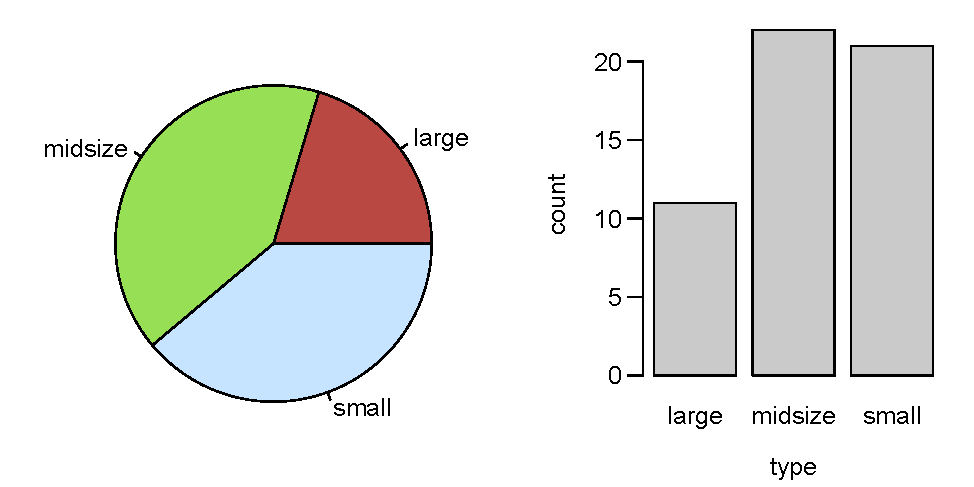
\includegraphics[height=2.1in]{ch1/carsTypePieChart/carsTypePieChart}
   \caption{A pie chart and bar plot of \var{type} for the data set \data{cars}.}
   \label{carsTypePieChart}
\end{figure}

\begin{exercise}
Using the pie chart, is it easy to tell which level, \resp{midsize} or \resp{small}, has a larger proportion in the sample? What about when using the bar plot?
\end{exercise}

\subsection{Comparing numerical data across groups}
\label{comparingAcrossGroups}

Some of the more interesting investigations can be considered by examining numerical data across groups. The methods required aren't really new. All that is required is to make a numerical plot for each group. Two convenient methods are introduced: side-by-side box plots and hollow histograms.

From the data set \data{cars}, we would like to compare vehicle price according to vehicle type. There are three levels of \var{type} (\resp{small}, \resp{midsize}, and \resp{large}), and the vehicle prices can be split into each of these groups, as shown in Table~\ref{carsPriceSplitByTypeTable}.
\begin{table}
\begin{center}
\begin{tabular}{ cc c cc c c }
  \cline{1-2} \cline{4-5}  \cline{7-7}
\multicolumn{2}{c}{\bf small} && \multicolumn{2}{c}{\bf midsize} && {\bf large} \\ 
  \cline{1-2} \cline{4-5}  \cline{7-7}
15900 & 11600 &\hspace{5mm}\ & 33900 & 28000 &\hspace{5mm}\ & 20800 \\ 
9200 & 10300 && 37700 & 35200 && 23700 \\ 
11300 & 11800 && 30000 & 34300 && 34700 \\ 
12200 & 9000 && 15700 & 61900 && 18800 \\ 
7400 & 11100 && 26300 & 14900 && 18400 \\ 
10100 & 8400 && 40100 & 26100 && 29500 \\ 
8400 & 10900 && 15900 & 21500 && 19300 \\ 
12100 & 8600 && 15600 & 16300 && 20900 \\ 
8000 & 9800 && 20200 & 18500 && 36100 \\ 
10000 & 9100 && 13900 & 18200 && 20700 \\ 
8300 &  && 47900 & 26700 && 24400 \\ 
  \cline{1-2} \cline{4-5}  \cline{7-7}
\end{tabular}
\end{center}
\caption{The variable \var{price} split up by \var{type}.}
\label{carsPriceSplitByTypeTable}
\end{table}

The \term{side-by-side box plot} is a traditional tool for comparing across groups, and it is shown in the left panel of Figure~\ref{carsPriceByTypeSBSandHH}. This is just three box plots -- one for each \var{type} -- squished into one plotting window and drawn on the same scale.
\begin{figure}
   \centering
   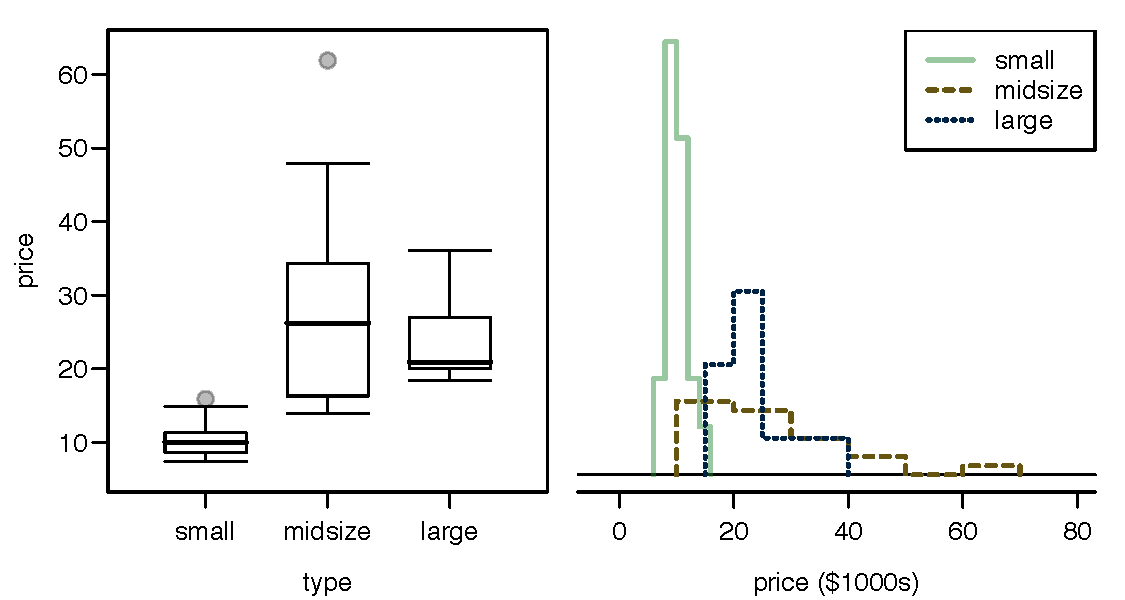
\includegraphics[width=5in]{ch1/carsPriceByTypeSBSandHH/carsPriceByTypeSBSandHH}
   \caption{Side-by-side box plot (left panel) and hollow histograms (right panel) for \var{price} where the groups are each level of \var{type}.}
   \label{carsPriceByTypeSBSandHH}
\end{figure}

Another plotting method worthy of mention is \term{hollow histograms}, which are just the histogram outlines of each group put on the same plot, as shown in the right panel of Figure~\ref{carsPriceByTypeSBSandHH}.

\begin{exercise} \label{comparingPriceByTypeExercise}
Use Figure~\ref{carsPriceByTypeSBSandHH} to compare the vehicle prices across groups. What do you notice about the approximate center of each group? What do you notice about the variability between groups? Is the shape relatively consistent between groups? How many \emph{prominent} modes are there for each group?
\end{exercise}

\begin{exercise}
What components of each plot in Figure~\ref{carsPriceByTypeSBSandHH} do you find most useful?
\end{exercise}



%%%%%
\section{Data collection}
\label{dataCollection}

The first step in conducting research is to identify topics or questions that are to be investigated. %This information is helpful in assessing what type of data must be collected. 
A clearly laid out research question is helpful in identifying what subjects or cases are to be studied and what variables are important. This information provides a foundation for \emph{what} data will be helpful. It is also important that we consider \emph{how} data is collected so that it is trustworthy. This section outlines important ideas and practices in data collection. %not only lays the groundwork for what data should be collected for research questions but also how to collect that data. This information is also helpful in evaluating the integrity of data collected by others.

%It is important to identify what information will most efficiently and accurately answer research questions prior to collecting data. To do so, the research questions that we hope to answer.

%\Comment{Describe components of the research question and how they influence what data to collect and how much to collect.}

%\Comment{Then we move onto data quality or ``trustworthy data and to judge the quality of data produced by others... careful design of data production is the most important prerequisite for trustworthy inference.'' (Moore \& McCabe, p192).}

%\subsection{Getting started}

%\Comment{First step is to identify both who/what is to be studied. This means identifying what people or things are to be sampled, and what data is to be collected about each case. Emphasize that this may be a difficult task and requires careful considerations. (MM192)}

%Here we consider two research questions important to many college students:
%\begin{itemize}
%\item Do folks who have a graduate degree earn more than those folks who without a graduate degree?
%\item Would a person maximize her income by obtaining a graduate degree or having additional outside experience?
%\end{itemize}
%These questions are similar in that they ask about the same variables: graduate education and income. However, the first only asks about what we observe in the population. The second asks what would happen under two different circumstances. To answer each question

%\subsection{Identifying an appropriate study method}

%Do folks who have college degree tend to make more money than folks who don't have a college degree? The research question considered here can be categorized as a \emph{What is?} question, and it can be answered by examining demographic data. Below are the average incomes for folks with and without a college degree in 2008:
%\begin{tabbing}
%\hspace{\parindent}  \= With a college degree: \=\hspace{8mm}\= \$ \\
%				\> Without a college degree: \>\>		    \$ \\
%\end{tabbing}
%\addvspace{-5mm}
%For people in the US, we can conclude that yes, folks with a college degree make more money on the average.

%We might ask a more interesting question: Is it more wise to pursue a college degree if the sole goal is to increase salary? After all, an additional four years of experience may be more valuable. Here we are asking a \emph{What if?} question. Would a person tend to do better or worse financially if she pursued a college degree? A first thought might be to say ``Yes, because look at the population data.'' However, perhaps it is not the college degree that actually caused those folks to have more money. Perhaps they would have even more money had they not gone to college. There is no way to answer this \emph{What if?} question using the summary statistics listed above.


% This is a much more difficult and complex question. The answer may be different from one individual to another individual,  also varies from one person to the other.

% What if the education of the same folks was actually different? Would we still observe the same set of folks, irregardless of their college education, averaging a higher income? Here we want to answer a were modified? What if a person had a chance to who had a college degree was able to go back in time and choose a different path?




%When we make a research question, it typically takes one of two forms:
%\begin{itemize}
%\item \textbf{What is?} Here we are interested in the current status or existing relationship between certain variables. Do folks who have college degree tend to have more money than folks who don't have a college degree? That is, is there an association between a person having a college degree and her net wealth?
%\item \textbf{What if?} When we ask \emph{What if?} we wonder, if we adjust one variable, does it affect the other? For instance, would a group of folks typically make more money if they earned a graduate degree than if they had not earned a graduate degree? Here we are not asking \emph{What is?} and instead are asking \emph{What if?}. % While this again asks about some connection between higher education and income, this research question runs deeper: is there a \emph{causal} connection between education and income?
%\end{itemize}
%When we ask a \emph{What is?} question, we are wondering whether two or more variables are naturally associated. %When we ask a \emph{What if?} question, we wonder whether one variable 


%Consider the following two research questions:
%\begin{itemize}
%\item If someone owns a Toyota vehicle, is she less likely to die from a heart attack?
%\item Are folks who take a daily aspirin less likely to die from a heart attack?
%\end{itemize}

% If we wanted to identify the exact  Here, a case represents a student who has enrolled in UCLA's undergraduate program. The population of interest is all students who have enrolled in UCLA's undergraduate program and have finished.

%Many research questions ask about the status of the world or to summarize characteristics of \emph{what is}.

%\Comment{Identifying the population or process of interest.}\\


%When we make a research question, we often try to answer it typically takes two forms:
%\begin{itemize}
%\item \textbf{What is?} Here we are interested in the current status or existing relationship between certain variables. For example, are folks who take a daily aspirin less likely to die from a heart attack? % folks with more education make more money? We collect \emph{observational data} to answer such questions. %are male or female possums longer, on average? These types of research questions about the \emph{natural order} of the world can be answered by collecting data from cases in some population. To determine if male or female possums are longer, we could collected a sample of possums from the population of all possums.
%\item \textbf{What if?} If turn a crank here, what happens over there? If a person  Does providing more education to a group of folks tend to cause an increase in their future income? To analyze such questions, we
%For instance, what if we gave heart-attack patients a new drug? Would it reduce their chance of death? In these types of questions, we would like to make some \emph{causal} connection. To provide convincing data that such a causal relationship exists, we must conduct an \emph{experiment}.
%\end{itemize}
%These two types of research questions are best answered by their own respective data collection technique.

%When we ask \emph{What is?}, we are often asking about connections between variables.

\subsection{Populations and samples}
\label{populationsAndSamples}

Consider the following three research questions:
\begin{enumerate}
\item What is the average mercury content in swordfish in the Atlantic Ocean?
\item\label{timeToGraduationQuestionForUCLAStudents} Over the last 5 years, what is the average time to degree for UCLA undergraduate students?
%how long has it taken students to complete their Ba
%How long does it take a student to complete a Bachelor's degree at your university? That is, what is the average time to degree?
%\item Of those students who graduate,  is the typical time to graduation for undergraduate students at UCLA? That is, what is the average number of years it takes a student at UCLA to earn her undergraduate degree?
%\item\label{textbooksAtAmazonOrSchoolPopulationQuestion} Are textbooks used in university classes typically cheaper on Amazon.com or at university bookstores?
%\item What is the average income of students who have graduated from my high school who did not go to college?
\item\label{identifyPopulationOfSulphinpyrazone} Does the drug sulphinpyrazone reduce the number of deaths in heart attack patients?
\end{enumerate}
In each research question, some population of cases is considered. In the first question, all swordfish in the Atlantic ocean are relevant to answering the question. Each fish represents a case, and all of these fish represent the \term{population} of cases. Often times, it is too expensive to collect data for ever case in a population. Instead a \emph{sample} is taken of the population. A \term{sample} represents a subset of the cases and often times represents only a small fraction of all cases in the population. For instance, 60 swordfish (or some other number) in the population might be selected, and this sample data may be used to provide an estimate of the population average, i.e. an answer to the research question. \\

\begin{exercise} \label{identifyingThePopulationForTwoQuestionsInPopAndSampSubsection}
For the second and third questions above, identify what is an individual case and also what is the population under consideration. Answers in the footnote\footnote{(\ref{timeToGraduationQuestionForUCLAStudents}) First, notice that this question is only relevant to students who complete their degree; the average cannot be computed using a student who never completes. Thus, only UCLA undergraduate students who have graduated in the last five years represent cases in the population under consideration. (\ref{identifyPopulationOfSulphinpyrazone}) A heart attack patient represents a case. The population represents all heart attack patients.}.
\end{exercise}


\subsection{Anecdotal evidence}

%\begin{quote}
%\emph{I can't believe Nixon won. I don't know anybody who voted for him.}
%\end{quote}

%\Comment{Find three examples where we might draw conclusions based on single events. MM examples: AIDS in young people must be common since we hear so much about it, flying seems more dangerous than driving because airplane crashes stick out in our minds, } \\

%\Comment{``Anecdotal evidence: Anecdotal evidence is based on haphazardly selected individual cases, which often come to our attention because they are striking in some way. These cases need not be representative of any larger group of cases.'' (MM193)} \\

We posed three research questions in Section~\ref{populationsAndSamples}. Below are some statements by folks who are responding to the research questions: % and conclusions based on those observations:
\begin{enumerate}
\item A man on the news got mercury poisoning from eating swordfish, so the average mercury concentration in swordfish must be dangerously high.
\item\label{iKnowThreeStudentsWhoTookMoreThan10YearsToGraduateAtUCLA} I met two students who took more than 10 years to graduate from UCLA, so it must take longer to graduate at UCLA than at many other colleges. %at least 8 years on average to graduate.
\item\label{myFriendsDadDiedAfterSulphinpyrazon} My friend's dad had a heart attack and died after they gave him sulphinpyrazone. The drug must not work.
\end{enumerate}
Each of the conclusions made are based on some data. However, there are two problems. First, the data described only represents a one or two cases. Secondly and more importantly, it is unclear whether these cases are actually representative of the population. Data collected in this haphazard fashion is called \term{anecdotal evidence}. \\

\begin{figure}
\begin{centering}
\includegraphics[width=60mm]{ch1/mnWinter/mnWinter}\hspace{4mm}
\begin{minipage}[b]{\textwidth - 64mm}
%The media regularly reports on striking stories that represent anecdotal evidence. 
\caption[anecdotal evidence]{In February 2010, some media pundits cited one large snow storm as valid evidence against global warming. As comedian Jon Stewart pointed out, ``It's one storm, in one region, of one country.''\footnote{www.openintro.org/clip/anecdotal.php}}%$^{\text{\fnsymbol{alwaysTwo}}}$}
%\footnote{http://www.thedailyshow.com/watch/wed-february-10-2010/unusually-large-snowstorm}}
%. \emph{TIME} reported a story with the headline \emph{Another Blizzard: What Happened to Global Warming?} However, the article actually explained took a reasonable position.)} %one web blog reported \emph{Washington DC covered in snow proves global warming wrong}.} %some television pundits cited unusually cold weather in the Northeast as strong evidence against the validity of global warming. Had they taken a Globally that same winter was the warmest on record (!).} % In a similar vein, a severe summer heat wave is sometimes cited as convincing evidence that global warming is real. }
\label{mnWinter}
\end{minipage}
\end{centering}
%\vspace{1mm}
%\rule{2in}{0.4pt} \\
%\footnotesize $^{\text{\fnsymbol{alwaysTwo}}}$http://www.thedailyshow.com/watch/wed-february-10-2010/unusually-large-snowstorm
\end{figure}


\begin{termBox}{\tBoxTitle{Anecdotal evidence}
Data collected in a haphazard fashion. Such evidence may be true and verifiable but often times represent extraordinary cases.}
\end{termBox}
%\begin{enumerate}
%\item 
%\end{enumerate}

% Additionally, each conclusion is based on only a few observations. 

Anecdotal evidence typically is composed of unusual cases that we recall based on their striking characteristics. For instance, we are more likely to remember the two folks we met who took 10 years to graduate than the six others who graduated in four years. %\\

%\begin{exercise}
%What is a conclusion you or someone you know has come to based on anecdotal evidence? Why did the data stick out in your mind?
%\end{exercise}

%\begin{exercise}
%Explain why the anecdotal cases described above in (\ref{myTextbooksAreMoreExpensiveOnAmazon}) and (\ref{myFriendsDadDiedAfterSulphinpyrazon}) are not necessarily representative of the populations you described in Exercise~\ref{identifyingThePopulationForTwoQuestionsInPopAndSampSubsection}. Answers in the footnote\footnote{(\ref{myTextbooksAreMoreExpensiveOnAmazon}) Maybe all English textbooks are cheaper at the UCLA Bookstore but the reverse is true of all other books. This small sample may not be representative of the population considered. (\ref{myFriendsDadDiedAfterSulphinpyrazon}) Such an emotional experience is easy to recall but may not be representative.}.
%\end{exercise}

Instead of looking at the most unusual cases, we often want to look at a sample that is representative of the population. It is also helpful to collect a sample with many cases.

\subsection{Sampling from a population}

The \data{cars} data set represents a {sample} of cars from 1993. All cars from 1993 represent the {population}, and the cars in the sample were \term{randomly} selected from the population. Randomly selected in this context is equivalent to a raffle to select cars. The name of each car from the population was written on a raffle ticket, and 54 tickets were drawn.
\begin{figure}[h]
\centering
\includegraphics[height=1.5in]{ch1/popToSample/popToSample}
\caption{Cars from the population are randomly selected to be included in the sample.}
\label{popToSample}
\end{figure}

Why pick a sample randomly? Why not just pick a sample by hand? Consider the following scenario. \\ %Suppose the cars were just picked by whatever cars were of greatest interest to the person doing the picking. \\

\begin{exercise}
Suppose a muscle car enthusiast is asked to select several cars for a study. What kind of cars do you think she might collect? Do you think her sample would be representative of all cars? %(b) Suppose you realize she might pick cars that reflect her taste if you ask her to pick cars that are representative of all cars? 
\end{exercise}

%Exercise~\ref{} suggests folks might not be very good at picking a representative sample. Even if a person tries very hard to pick a sample representing the population, she might neglect some component that is important.

Even If someone was permitted to pick and choose exactly which cars were included in the sample, it is entirely possible that the sample could be skewed to that person's interests, which may be entirely unintentional. This introduces \term{bias} into a sample.
\begin{figure}[h]
\centering
\includegraphics[height=1.5in]{ch1/popToSample/popToSubSample}
\caption{Instead of sampling from all cars from 1993, an environmentalist might inadvertently pick cars with high mileage disproportionally often.}
\label{popToSubSample}
\end{figure}
Sampling randomly helps resolve this problem. The most basic random sample is called a \term{simple random sample}, and is the equivalent of using a raffle to pick the sample. This means that each case in the population has an equal chance of being included and there is no implied connection between the cases in the sample. The act of taking a simple random sample helps eliminate bias, however, it can still crop up in other ways.

Even when people are seemingly picked at random (for surveys, etc.), caution must be exercised if the \term{non-response} is high. For instance, if only 15\% of the people randomly sampled for a survey actually respond, then it is unclear whether the results are \term{representative} of the rest of the population of interest. \term{Non-response bias} can skew results one way or another\footnote{In major polling outfits such as Gallup, researchers try to keep the non-response level low while also making corrections to attempt to offset any lingering bias. These types of corrections are beyond the scope of this text.}.
\begin{figure}[h]
\centering
\includegraphics[height=1.5in]{ch1/popToSample/surveySample}
\caption{Surveys may result in only reaching a certain group within the population, and it is not obvious how to fix this problem.}
\label{surveySample}
\end{figure}

Another common downfall is a \term{convenience sample}, where individuals who are easily accessible are more likely to be included in the sample. For instance, if a political survey is done by stopping people walking in the Bronx, this probably will not fairly represent all of New York City. It is often difficult to discern what sub-population a convenience sample represents. \\

\begin{exercise}
We can easily access ratings for products, sellers, and companies through websites. These ratings are based only on those people who go out of their way to provide a rating. If a seller has a rating of 95\% on Amazon, do you think this number might be artificially low or high? %\footnote{For your consideration, one of the authors of this book has sold 67 items on Amazon and only received 16 ratings based on these transactions.}?
Why?
%If you stand outside your school's student union to survey people who walk by, what sub-population do you think you are sampling? How would this sub-population be different from the population of the city?
\end{exercise}


%\Comment{Propose two sampling methods, one a convenience sample and one a simple random sample.} \\

%\begin{exercise}
%\Comment{Ask the reader to decide which sample is more trustworthy.}
%\end{exercise}

%\Comment{Formally define \term{convenience sample} and \term{bias} (possibly use phrase ``not representative''). Describe how bias can be generated from non-random samples.}

%\Comment{Propose random sampling as best technique to ensure the data isn't biased. Define \term{simple random sample}.}

%\Comment{Note that sampling techniques extend beyond a simple random sample, though all the best incorporate some method where cases are selected at random.}

%\subsection{Collecting a sample}

%\Comment{Deciding how many cases to sample or how to form groups (MM193).}

%\subsection{Experiments}

%\subsection{Randomized experiments}


%\section{Observational studies and experiments}
%\label{obsExp}

\subsection{Explanatory and response variables}
\label{explanatoryAndResponse}

%Beyond looking at whether variables are associated in some way, it is useful to examine the underlying nature of that association. In particular, does association always imply causation? (No.) %Beyond what the data look like, it is important to ask: how was the data collected? In this section, this question is examined carefully, and the answer to this question affects what interpretations can be drawn from the data. Not all data are collected equally!

Consider the second question from page~\pageref{possibleCausationQuestionForPossums} for the \data{possum} data set:
\begin{enumerate}
\item[(2)] Will males or females, on the average, be longer?
\end{enumerate}
This question might stem from the belief that \var{sex} would affect \var{totalL} but not the reverse. If \var{sex} is suspected to affect the total length, then \var{sex} is the \term{explanatory} variable and \var{totalL} is the \term{response} variable in the relationship\footnote{Sometimes the explanatory variable is called the \term{independent} variable and the response variable is called the \term{dependent} variable. However, this becomes confusing since a \emph{pair} of variables might be independent or dependent, so we avoid this language.}. If there are many variables, it may be possible to label a number of them as explanatory and the others as response variables.

\begin{tipBox}{\tipBoxTitle{Explanatory and response variables}
To identify the explanatory variable in a pair of variables, identify which of the two is suspected of affecting the other.

\hspace{6mm}\includegraphics[height=0.4in]{ch1/expResp/expResp}}
\end{tipBox}

\begin{exercise}
Would you suspect having a larger head length might cause a change in skull width? Or could the \emph{causal} relationship be the reverse? Does it make sense to discuss causation here?
\end{exercise}

\begin{caution}{association does not imply causation}{Labeling variables as \emph{explanatory} and \emph{response} does not guarantee the relationship between the two is actually causal, even if there is an association identified between the two variables. We use these labels only to keep track of which variable we suspect affects the other.}
\end{caution}

In some cases, there is no explanatory or response variable. Consider the first question from page~\pageref{possumHeadSizeQuestion}:
\begin{enumerate}
\item[(1)] If a possum has a shorter-than-average head, do you think its skull width will be smaller or larger than the average skull width?
\end{enumerate}
This question does not have an explanatory variable since it doesn't really make sense that \var{headL} would affect \var{skullW} or vice-versa, i.e. the direction is ambiguous.

%Consider the variables \var{headL} and \var{skullW} from the \data{possum} data set. A scatterplot of these variables is given in Figure~\vref{possumHeadVsSkullW}, which shows a positive association between the variables. However, it is not clear that a possum having a long skull would \emph{cause} the possum to have a wide skull, or vice versa. Instead, these variables might both be caused to vary together due to another variable such as \var{age}, \var{gender}, or an unobserved variable.

\subsection{Experiments}
\label{experiments}

An association between two variables means they are in some way connected. It would be useful to expand on this connection and say that one variable causes the other to change, however, it is not clear that is always the case. When is such a conclusion reasonable?

Consider the variables \var{pop} (living location) and \var{sex}, summarized in Table~\ref{possumPopSexContTableRowProps} using row proportions. The data suggests there might be a difference: 67\% of the sample was male for \resp{other} while only 48\% was male for \resp{Vic}. Suppose these proportions were the same in the population as in the sample, i.e. that there was a real difference in gender ratio in the two geographical regions\footnote{The biological mechanism for gender suggests the ratio should always be one male to every one female, however, the animals that actually survive might not do so in a one-to-one ratio and other factors may also play into the resulting proportion of males in a population.}.
\begin{table}[ht]
\begin{center}
\begin{tabular}{rrr}
  \hline
 & female & male \\ 
  \hline
  Victoria    & 0.52 & 0.48 \\ 
  other & 0.33 & 0.67 \\ 
   \hline
\end{tabular}
\end{center}
\caption{Contingency table with row proportions of possums' sex based on location.}
\label{possumPopSexContTableRowProps}
\end{table}

\begin{exercise}\label{popSexExplanatoryResponse}
If we suspect that \var{pop} affects \var{sex} in possums, which variable would be the explanatory variable and which the response?
\end{exercise}

Does Exercise~\exer{popSexExplanatoryResponse} imply that living in New South Wales or Queensland  \emph{causes} a possum to be male more often than it would in Victoria? Put it another way: if possums were transported from Victoria to New South Wales or Queensland, does this actually mean their offspring is more likely to be male than if it had been born in Victoria? The data doesn't answer this \emph{causal} question.

To answer whether living location does affect gender, it would be interesting to take bunch of possums and try it out:
\begin{itemize}
\item Collect a random sample of 100 possums from Victoria (or as best a random sample as is possible).
\item Randomly split the 100 possums into two groups. Leave one group in Victoria and transport the other group to New South Wales and Queensland.
\item Observe the offspring of each group.
\end{itemize}
%This setup is called an \term{experiment} because the possum locations -- the explanatory variable -- are not simply observed but are imposed by the researchers. More accurately, this would be a \term{randomized experiment} because each possum was randomly assigned its group.
This study is called an \term{experiment} because the possum locations -- the explanatory variable -- are not simply observed but are %determined by random chance
imposed on the possums by the researchers in this setup. Furthermore, the group assignments are randomly generated through the equivalent of a raffle, making this a \term{randomized experiment}. %would be \emph{randomly} assigned to prevent any inadvertant bias for the same reasons

If there is a big difference in these two groups again in the experiment, then it would seem reasonable to conclude that living in New South Wales and Queensland actually \emph{causes} more males to be born and survive. If that difference seems to disappear or be minor, then living in New South Wales and Queensland may not cause more male possums to survive to adulthood but may just be \emph{associated} with more males surviving. That is, it might be true that the variables really are associated, however, they may not share a causal relationship.

\begin{tipBox}{\tipBoxTitle{association $\neq$ causation}
In general, association does not imply causation, and causation can only be inferred from an experiment.}
\end{tipBox}

%An experiment offers the most straightforward way of testing the hypothesis of causality. Within the many steps of completing an experiment, there are three key concepts: \textbf{control} for lurking variables, \textbf{randomize} how the experimental groups are setup, and \textbf{replicate} the experiment many times, typically by including many subjects in the experiment. A general experiment might proceed as follows:
%\begin{enumerate}
%\item[(1)] \textbf{ID the relationship of interest.} Identify the explanatory and response variables of interest.
%\item[(2)] \textbf{ID the population, take a sample.} Identify the population of interest, and collect a random sample from this population. If the 
%\item[(3)] \textbf{Randomize.} Randomly split the sample into groups, one group for each level of the explanatory variable. For the possum study, there were two groups since there were two levels of \var{pop}: \resp{Vic} and \resp{other}.
%\item[(4)] Observe and record the response variable for each subject in each group. For the possum experiment, this meant observing the gender of each offspring in each group.
%\item[(5)] Analyze the data and look for a \emph{convincing} difference in the response variable in each group\footnote{What describes a \emph{convincing} difference will be discussed in Chapter~\ref{foundationsForInference}.}. When such a difference exists, it is (often) reasonable to conclude that there is a causal relationship.
%\end{enumerate}
%The randomization in step (3) does not guarantee bias has been eliminated in the experiment but it is a simple and important first step in reducing bias. Some forms of bias in experiments with human subjects\footnote{Human subjects are more often called \term{patients}, \term{volunteers}, or \term{study participants}.} them will be discussed in Section~\ref{biasInHumanExperiments}.

%An experiment offers the most straightforward way to test the hypothesis of causality. Within the many steps of completing an experiment, there are three key concepts: \textit{control} for lurking variables, \textit{randomize} how the experimental groups are setup, and \textit{replicate} the experiment many times, typically by including many subjects in the experiment. A general experiment might proceed as follows:
%\begin{enumerate}
%\item[(1)] Identify the explanatory and response variables of interest.
%\item[(2)] \textbf{Replicate.} Collect a random sample of many subjects from the population of interest.
%\item[(3)] \textbf{Randomize.} Randomly split the sample into groups, one group for each level of the explanatory variable. %For the possum study, there were two groups since there were two levels of \var{pop}: \resp{Vic} and \resp{other}.
%\item[(4)] Observe and record the response variable for each subject in each group. %For the possum experiment, this meant observing the gender of each offspring in each group.
%\item[(5)] Analyze the data and look for a \emph{convincing} difference in the response variable in each group\footnote{What describes a \emph{convincing} difference will be discussed in Chapter~\ref{foundationsForInference}.}. When such a difference exists, it is (often) reasonable to conclude that there is a causal relationship.
%\end{enumerate}
%The \textbf{control} step must be considered throughout. For the hypothetical possum experiment, it may be important to note which possums were siblings and include this information in the data analysis\footnote{For some species, there can be correlations in gender between siblings.}. If the experiment had human subjects\footnote{Human subjects are more often called \term{patients}, \term{volunteers}, or \term{study participants}.}, there are several strategies to control lurking variables and these will be discussed in Section~\ref{biasInHumanExperiments}.

%An experiment offers the most straightforward way of testing the hypothesis of causality. There are several steps to running an experiment:
%\begin{enumerate}
%\item[(1)] Identify the explanatory and response variables of interest. Obtain a sample of study \term{subjects} (e.g. 100 possums).
%\item[(2)] Randomly split up the study subjects into groups, one group for each level of the explanatory variable. For the possum study, there were two groups since there were two levels of \var{pop}: \resp{Vic} and \resp{other}.
%\item[(3)] Observe and record the response variable for each subject in each group. For the possum experiment, this meant observing the gender of each offspring in each group.
%\item[(4)] Analyze the data and look for a \emph{convincing} difference in the response variable in each group\footnote{What describes a \emph{convincing} difference will be discussed in Chapter~\ref{foundationsForInference}.}. When such a difference exists, it is (often) reasonable to conclude that there is a causal relationship.
%\end{enumerate}
%The randomization in step (2) does not guarantee bias has been eliminated in the experiment but it is a simple and important first step in reducing bias. Some forms of bias in experiments with human subjects\footnote{Human subjects are more often called \term{patients}, \term{volunteers}, or \term{study participants}.} them will be discussed in Section~\ref{biasInHumanExperiments}.

\begin{tipBox}{\tipBoxTitle{Three experimental design principles}

%\textbf{Control.} Control the value of the explanatory variable in each case or trial, and control the effects of other potentially influential variables.

\textbf{Control.} Control the value of the explanatory variable in each case, and control the effects of other potentially influential variables.

\vspace{0.3cm}
\textbf{Randomize.} Use \term{subjects} (i.e. cases) from a random sample of the population when possible. Subjects should be randomly split into groups, where groups are based on the explanatory variable.

%\textbf{Randomize.} Use \term{subjects} (i.e. cases) from a random sample of the population when possible. Each subject should be randomly assigned into a group, where groups are based on the explanatory variable.

%\textbf{Randomize.} Use \term{subjects} (i.e. cases) from a random sample of the population when possible. Each case should be randomly assigned into a group, where groups are based on the explanatory variable.

%\textbf{Randomize.} Use study \term{subjects} (i.e. cases) from a random sample of the population. In an experiment, subjects should be randomly split into groups, one group for each level of the explanatory variable.

\vspace{0.3cm}
\textbf{Replicate.} Observe many cases or run many trials.}
\end{tipBox}

Controlling variables that might affect both the explanatory variable and response may be the most difficult part of an experiment because such variables are difficult to identify. For instance, it would be appropriate to control for (take into account) which possums are siblings in an analysis of the hypothetical possum experiment. In an experiment with human subjects\footnote{Human subjects are more often called \term{patients}, \term{volunteers}, or \term{study participants}.}, there are complex factors to control for, and these will be discussed in more detail in Section~\ref{biasInHumanExperiments}.

If study subjects are not from a random sample of the population, additional justification is needed to extend an experiment's conclusions to the population.

\begin{exercise}
Describe how the three experimental principles fit into the hypothetical possum experiment.
\end{exercise}

%An experiment offers the most straightforward way to test the hypothesis of causality and there are several steps to running an experiment:
%\begin{enumerate}
%\item[(1)] Obtain a sample of \term{study subjects} (e.g. 100 possums) from the population of interest.
%\item[(2)] Randomly split up the study subjects into groups, one group for each level of the explanatory variable.
%\item[(3)] Observe and record the response variable for each subject in each group.
%\item[(4)] Analyze the data to evaluate whether there was an effect on the response based on the group.
%\end{enumerate}
%There are three key components to an experiment. First, \textit{randomization} is used to reduce bias in the data. Second, the experiment is \textit{replicated} many times by using many study subjects\footnote{In engineering applications, replications of an experiment might be called \term{replicates} instead of \textit{study subjects}.}. Lastly, lurking variables must be \textit{controlled}. Controlling lurking variables may be the most difficult part of an experiment because it may come into play in several steps. For instance, it would be appropriate to control for (take into account) which possums are siblings in an analysis of the hypothetical possum experiment. In an experiment with human subjects\footnote{Human subjects are more often called \term{patients}, \term{volunteers}, or \term{study participants}.}, there are many factors to control for, and these will be discussed in more detail in Section~\ref{biasInHumanExperiments}.

\subsection{Observational studies}

The \data{possum} data set was actually from an \term{observational study} since the researchers did not randomly assign which possums lived where. Generally, data in observational studies is collected only by monitoring what occurs while experiments require the explanatory variable to be assigned for each subject by the researchers.

Inferring causal conclusions from experiments is often reasonable, however, making the same causal conclusions from observational data can be treacherous and is not recommended. Thus, we can generally only infer associations from observational data.

\begin{exercise} \label{sunscreenLurkingExample}
Suppose an observation study tracked sunscreen use and skin cancer and it was found that the more sunscreen someone used, the more likely they were to have skin cancer (!). Does this mean sunscreen \emph{causes} skin cancer?
\end{exercise}

Exercise~\exer{sunscreenLurkingExample} has a missing variable: sun exposure. If someone is out in the sun all day, she is more likely to use sunscreen \emph{and} more likely to get skin cancer.
\begin{center}
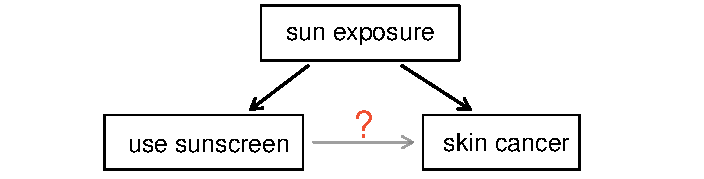
\includegraphics[height=1.0in]{ch1/variables/sunCausesCancer}
\end{center}
It just so happens that if someone is exposed to the sun they also usually use sunscreen. Exposure to the sun is unaccounted for in the investigation, giving the incorrect impression that sunscreen causes skin cancer.

Sun exposure is what is called a \term{lurking variable}, which is a variable that is the true cause for change in the response. While one method to justify making causal conclusions from observational studies is to exhaust the search for lurking variables, there is no guarantee that all lurking variables can be examined or measured.

In the same way, the \data{possum} data set is an observational study with possible lurking variables of its own, and its data cannot easily be used to make causal conclusions.

\begin{exercise}
There appears to be a real difference in the proportion of possums that are male based on location. However, it is unreasonable to conclude that this is a causal relationship because the data is observational. Suggest at least one lurking variables that might be the true cause for the change in \var{sex}. One lurking variable is listed in the footnote\footnote{Some genes can affect one gender more than the other. If the \resp{other} population has a gene that affects males more positively than females and this gene is less common in the \resp{Vic} population, this might explain the difference in gender ratio for each level of \var{pop}.}.
\end{exercise}

\subsection{Reducing bias in human experiments}
\label{biasInHumanExperiments}

Randomized experiments are the gold standard for data collection but do not ensure an unbiased perspective into the cause and effect relationships in all cases. Human studies are perfect examples where bias can unintentionally arise. Here we reconsider the sulphinpyrazone study, which was described at the beginning of this chapter. %Let's look at a study that examines the benefits of a drug on reducing deaths from heart attacks.

Researchers wanted to examine whether a drug called sulphinpyrazone would reduce the number of deaths after heart attacks. They designed an experiment because they wanted to draw causal conclusions about the drug's effect. Study volunteers were randomly placed into two study groups. One group, the \term{treatment group}, received the drug. The other group, called the \term{control group}, did not receive any drug treatment.

Put yourself in the place of a person in the study. If you are in the treatment group, you are given a fancy new drug that you anticipate will help you. On the other hand, a person in the other group doesn't receive the drug and sits idly, hoping her participation doesn't increase her risk of death. These perspectives suggest there are actually two effects: the one of interest is the effectiveness of the drug and the second is an emotional effect that is difficult to quantify.

Researchers aren't interested in this emotional effect, which might bias the study. To circumvent this problem, researchers do not want patients to know which group they are in. When researchers keep the patients in the dark about their treatment, the study is said to be \term{blind}. But there is one problem: if a patient doesn't receive a treatment, she will know she is in the control group. The solution to this problem is to give fake treatments to patients in the control group. A fake treatment is called a \term{placebo}, and an effective placebo is the key to making a study truly blind. A classic example of a placebo is a sugar pill that is made to look like the actual treatment pill. Often times, a placebo results in a slight but real improvement in patients. This often positive effect has been dubbed the \term{placebo effect}.

% Researchers aren�t interested in this emotional effect, which might bias the study, although it is not entirely obvious which way the bias would be. There are two methods to reduce or eliminate the bias. First, give the patients in the control group a fake treatment, which is called a placebo. Usually this is just a sugar pill that looks like the real drug. Then, for this placebo to eliminate this emotional effect, don�t tell any of the patients if they are receiving the real drug or the placebo so all are under the same emotional condition. In this setup, the study is said to be \term{blind} since no patients know their treatment. Findings suggest patients in control groups respond differently when the study is blinded to when it is not, and this effect  that the placebo is eliminating is aptly named the \term{placebo effect}.

The patients are not the only ones who should be blinded: doctors and researchers can accidentally bias a study. When a doctor knows a patient has been given the real treatment, she might inadvertently give that patient more attention or care than a patient that she knows is on the placebo. To guard against this bias (which again has been found to have a measurable effect in some instances), most modern studies employ a \term{double-blind} setup where doctors or researchers who interact with patients are, just like the patients, unaware of who is or is not receiving the treatment\footnote{There are always some researchers involved in the study who do know which patients are receiving which treatment, however, they do not have interactions with the patients and do not tell the \emph{blinded} doctors who is receiving which treatment.}.

\subsection{Variability within data}
\label{variabilityWithinData}

The study examining the effect of sulphinpyrazone was double-blinded, and the results are summarized in Table~\ref{sulphinpyrazoneResults}. The variables have been called \var{group} and \var{outcome}. Do these results mean the drug was effective at reducing deaths? In the observed groups, a smaller proportion of individuals died in the treatment group than the control group (0.056 versus 0.081), however, it is unclear whether that difference is \emph{convincing evidence} that the drug is effective.
\begin{table}[ht]
\begin{center}
\begin{tabular}{l l cc rr}
& & \multicolumn{2}{c}{\var{outcome}} \\
  \cline{3-4}
		&			& 	\resp{lived} 	& \resp{died} & Total & \hspace{3mm}  \\ 
  \cline{2-5}
		&	\resp{treatment} 	& 692    		& 41   & 733  	 \\ 
  \raisebox{1.5ex}[0pt]{\var{group}}		&	\resp{control} 	& 682    		& 60     & 742	 \\ 
  \cline{2-5}
  		&	Total		& 1374	& 101	&  1475 \\
  \cline{2-5}
\end{tabular}
\end{center}
\vspace{-2mm}
\caption{Summary results for the sulphinpyrazone study.}
\label{sulphinpyrazoneResults}
\end{table}

\begin{example}{Suppose there had been only 45 deaths in the control group. Would this be convincing evidence that the drug was effective?} \label{45PlaceboDeaths}
The proportion is still in favor of the drug (0.056 versus 0.061), however, this minor difference is not very convincing. The sample proportion is rarely \emph{exactly} equal to what will happen with all heart attack victims. The sample only provides an \emph{estimate}.
\end{example}

Example~\exam{45PlaceboDeaths} is a reminder that the sample will not perfectly reflect the population. It is possible to see a small difference \emph{by chance}. Small differences in large samples can be important and meaningful but it is unclear when we should say that a difference is so large it was probably not due to chance. In Section~\ref{caseStudyOfSulphinpyrazone}, we evaluate whether Table~\ref{sulphinpyrazoneResults} shows convincing evidence that sulphinpyrazone is effective at reducing deaths or whether we remain unconvinced. %the difference of 2.5\% in the death rates was due to chance. %Chapter~\ref{foundationsForInference} provides a more general and rigorous framework to form conclusions based on data.

\section{Case study: efficacy of sulphinpyrazone*}
\label{caseStudyOfSulphinpyrazone}

%In this section, we examine a case study. In Chapter~\ref{foundationsForInference}, we will revisit these topics in greater detail

\begin{example}{Suppose your professor splits the students in the front row into two groups: students on the left and students on the right. If $\bar{x}_{_L}$ and $\bar{x}_{_R}$ represent the mean height of students on the left and right, respectively, would you be surprised if $\bar{x}_{_L}$ did not {exactly} equal $\bar{x}_{_R}$?}\label{classRightLeftSideForHeight}
While the mean heights would probably be close to each other, it would be unusual for them to be exactly the same. We would probably observe a small difference due to {chance}.
\end{example}

\begin{exercise}
If we don't think the side of the room a person sits on is related to her height, what assumption are we making about the relationship of the variables \var{height} and \var{sideOfRoom}? Answer in the footnote\footnote{The variables \var{height} and \var{sideOfRoom} are independent.}.
\end{exercise}

Table~\ref{sulphinpyrazoneResults} shows there were 19 fewer deaths in the treatment group than in the control group for the sulphinpyrazone study, a difference in death rates of 2.5\% $\left( \frac{60}{742} - \frac{41}{733} = 0.025 \right)$. %Is it plausible that this difference is due to chance and the drug actually had no effect on the patient outcome? Or i
Might this difference just be due to chance? Or is this convincing evidence that sulphinpyrazone works? We label these two competing claims, $H_0$ and $H_A$:
\begin{itemize}
\item[$H_0$] \textbf{Independence model.} The variables \var{group} and \var{outcome} are independent. They have no relationship, and the difference in death rates, 2.5\%, was due to chance.
\item[$H_A$] \textbf{Alternate model.} The \var{group} and \var{outcome} variables are \emph{not} independent. The difference in death rates of 2.5\% was not due to chance and the treatment did reduce the death rate.
\end{itemize}

%In Example~\exam{classRightLeftSideForHeight}, it was acknowledged that the mean heights of two groups will be about the same, however, they are rarely \emph{exactly} the same. The important question for the sylphinpyrazone study is, Is the difference 19 so large that it does not seem reasonable for the variables to be independent?

Consider what it would mean to the study if the independence model, which says that the variables \var{group} and \var{outcome} are unrelated, is true. Each person was either going to live or die, and the drug had no effect on the outcome. The researchers were just randomly splitting up these individuals into two groups, just like we split the first row of the class in half in Example~\exam{classRightLeftSideForHeight}. The researchers observed a difference of 2.5\% by chance.

Consider the alternative: the treatment affected the outcome. We would expect to see some difference in the groups, with a lower percentage of deaths in the group of patients who received the drug.

If the data conflicts so much with $H_0$ that the independence model cannot be deemed reasonable, we will reject it in favor the alternate model, $H_A$. In other words, we will not reject the position that $H_0$ is true unless the evidence from the study in favor of $H_A$ is too convincing.

\subsection{Simulating the study*}

%The independence model, $H_0$ , says that the variables trmt and outcome are unrelated. If this is true, it means that each person was either going to live or die and the drug had no e?ect on the outcome. Under this setup, the researchers were just randomly splitting up these individuals into two groups, the treatment and control groups, and we would expect the death rates in each group to be about the same; the di?erence in death rates should be approximately zero. We observed a di?erence of 2.5\%, and we want to determine if a di?erence this large is plausibly due to chance. 

%If the alternative model is true, we anticipate some difference. However, if the independence model is true, we know we would expect a difference near 0. We can use \term{simulations} to determine how close we would expect our difference to be to 0.
Suppose $H_0$ is true. The researchers had split the patients in the study randomly into the two groups and observed the difference. Under this model, the 2.5\% difference was due to chance.

We can simulate differences due to chance using a \term{randomization technique}. If we randomly assign each person in the study into either a fake treatment or fake control group, we observe such a difference. We do this by taking 733 \resp{treatmentFake} and 742 \resp{controlFake} labels\footnote{These label counts correspond to the number of \var{treatment} and \var{control} assignments in the actual study.} and randomly assign them to the patients. Because these assignments are made independent of the outcomes, any difference in these fake groups is due to chance.
%If the independence model, $H_0$ , were true, we can randomly split the patients into two groups, just like the researchers. If we do this, we are simulating the experiment and see what di?erences we might get if $H_0$ is true. 
%Imagine wWe do this by taking 733 \resp{drug} and 742 \resp{placebo} labels, and we randomly give them to each patient. If $H_0$ is true, we have split all the patients into two random groups, just like the researchers. Now we can determine the difference in death rates between the two groups, which we know is by chance.
If we do this simulation many times, we get an idea for what represents common differences under the independence model, and we can evaluate whether the observed difference, 2.5\%, is too big to plausibly be due to chance.
\begin{center}
Independence model \\
$\downarrow$ \\
differences due to chance
\end{center}
If 2.5\% is an uncommonly large difference from the independence model, then we would conclude that this model does not fit our data and we reject $H_0$ in favor of $H_A$, that the drug is actually effective.

We use a computer program to randomly assign these labels to the patients. A contingency table representing results from such a randomization is shown in Table~\ref{sulphinpyrazoneRand1}. \\
\begin{table}[ht]
\begin{center}
\begin{tabular}{l l cc rr}
& & \multicolumn{2}{c}{\var{outcome}} \\
  \cline{3-4}
		&			& 	\resp{lived} 	& \resp{died} & Total & \hspace{3mm}  \\ 
  \cline{2-5}
		&	\resp{treatmentFake} 					& 686    		& 47    & 733 	 \\ 
  \raisebox{1.5ex}[0pt]{\var{groupFake}}		&	\resp{controlFake} 	& 688    		& 54 & 742    	 \\ 
  \cline{2-5}
\end{tabular}
\end{center}
\caption{Simulation results, where any difference in death rates between \resp{treatmentFake} and \resp{controlFake} is purely due to chance.}
\label{sulphinpyrazoneRand1}
\end{table}
% and see how big of a difference we get under this model. Table~\ref{sulphinpyrazoneDF} shows persons 1, 2, and 1475. To run this simulation, we suppose each person was either going to live or die. That is, we fix \var{outcome} for each person. Then we do what the researchers did: we randomize their treatments. This randomization just means a random reordering of the variable \var{treatment}. A contingency table with the results of such a randomization is shown in Table~\ref{sulphinpyrazoneRand1}. \\

\begin{exercise} \label{sampleDifferenceInDrugAndPlaceboGroupSulph}
What is the difference in death rates between the two fake groups in Table~\ref{sulphinpyrazoneRand1}? How does this compare to the observed 2.5\% in the real groups? Answer in the footnote\footnote{$54/742 - 47/733=0.0087$ or about 0.9\%. This difference due to chance is smaller, however, we should run more simulations to get a good idea of what difference we get by chance, i.e. it is possible 0.9\% was a fluke.}.
\end{exercise}

\subsection{Checking for independence*}

We computed one possible difference under the independence model in Exercise~\exer{sampleDifferenceInDrugAndPlaceboGroupSulph}, which represents the results of one simulation. We want to repeat the simulation many more times to get a good idea of what represents a difference due to chance. Figure~\ref{sulphRandHist} shows a histogram of the differences found from 100 simulations. \\
 \begin{figure}
    \centering
    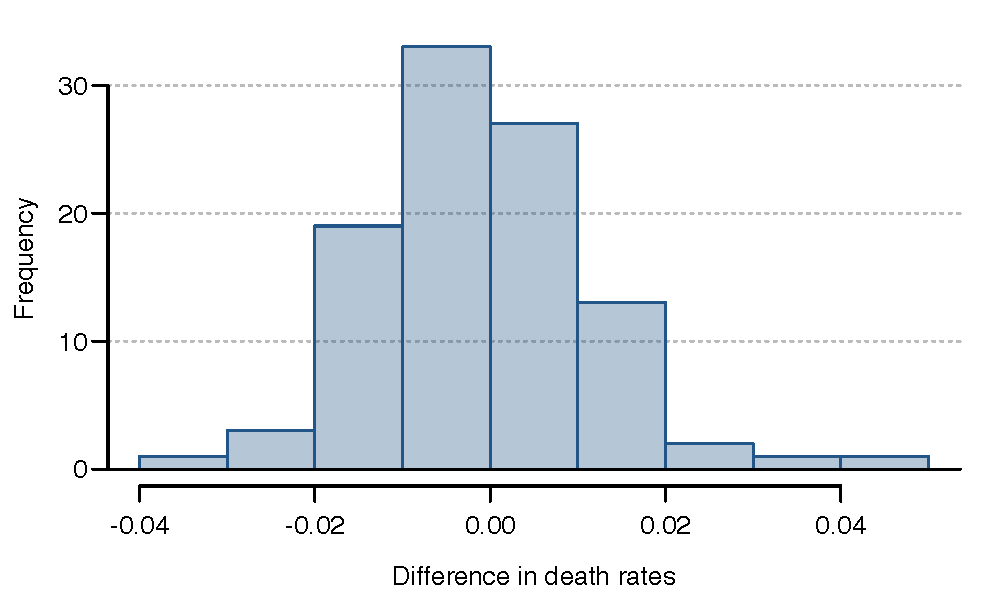
\includegraphics[height=2in]{ch1/sulphRandHist/sulphRandHist}
    \caption{A histogram of differences from 100 simulations produced under the independence model, $H_0$, where \var{groupFake} and \var{outcome} are independent. Four of the one-hundred simulations had a difference of at least 2.5\%.}
    \label{sulphRandHist}
 \end{figure}
 
\begin{example}{Consider the observed difference in the data, 2.5\%. Does this difference appear to be just another regular observation in the histogram shown in Figure~\ref{sulphRandHist}?}\label{isThe2Point5DifferenceDueToChance}
If the independence model were true, then 2.5\% is pretty large relative to most observations. Only 4\% of the simulated differences were at least as large, suggesting an observation this large is relatively uncommon and probably not due to chance. We reject the independence model and conclude the drug actually did reduce deaths. (If you think a 4\% chance is not very unusual, you might answer differently.)
\end{example}

One field of statistics is built on evaluating whether such differences are due to chance: statistical inference. In statistical inference, statisticians evaluate which model is most reasonable given the data. Errors do occur: we might choose the wrong model. While we do not always choose correctly, statistical inference gives us tools to control and evaluate how often these errors occur. In Chapter~4%\ref{foundationsForInference} ZZQ
, we give a formal introduction to the problem of model selection. However, we spend the next two chapters building a foundation of probability and theory necessary to make that discussion rigorous.

%\begin{exercise}
%Suppose you rejected $H_0$ in favor of $H_A$ in Exercise~\exer{isThe2Point5DifferenceDueToChance} as in the prop, could it be possible you made an error? What would be the implications of this error? Answer in the footnote\footnote{It is possible the variables are in fact independent.}.
%\end{exercise}










